\documentclass[10pt]{article}
\setlength{\emergencystretch}{2em}
\usepackage[utf8]{inputenc}
\usepackage[T1]{fontenc}
\usepackage{lmodern}
\usepackage{amsmath,mathtools,amssymb,amsfonts,amsthm,mathrsfs,bm}
\usepackage[dvipsnames]{xcolor}
\usepackage{graphicx,placeins,booktabs,array,tabularx,enumitem,seqsplit,tikz}
\usetikzlibrary{arrows.meta,decorations.pathmorphing,decorations.markings,patterns,positioning,calc}
\usepackage{footmisc}
\usepackage{cite,microtype}
\usepackage[colorlinks=true,citecolor=Blue,linkcolor=Blue,urlcolor=Blue]{hyperref}
\usepackage[labelfont={small,bf,sf},textfont={small,sf}]{caption}
\usepackage{authblk}
\usepackage[in]{fullpage}

\hypersetup{
  breaklinks=true,
  pdftitle={A universal sign law and slice real-rootedness for even-order multivalued group polynomials},
  pdfauthor={Atharvsinh Jadav}
}

\numberwithin{equation}{section}
\allowdisplaybreaks[1]
\pdfpageheight 11in
\pdfpagewidth 8.5in
\textheight 9in
\setlength\parskip{2.8pt plus 2pt minus .9pt}
\clubpenalty=2000
\widowpenalty=2000
\displaywidowpenalty=2000
\setlength{\intextsep}{11pt plus 2pt minus 2pt}
\setlength{\textfloatsep}{15pt plus 3pt minus 4pt}

% Muted publication color palette for TikZ diagrams
\definecolor{pBlue}{HTML}{285E7B}
\definecolor{pBlueFill}{HTML}{EAF2F6}
\definecolor{pGreen}{HTML}{4D7D55}
\definecolor{pGreenFill}{HTML}{ECF4EE}
\definecolor{pRed}{HTML}{AA3038}
\definecolor{pRedFill}{HTML}{F7E9EA}
\definecolor{pOrange}{HTML}{B86A2E}
\definecolor{pOrangeFill}{HTML}{FDF2E9}
\definecolor{pGray}{HTML}{555555}
\definecolor{pLight}{HTML}{F4F5F7}

% Theorem environments
\theoremstyle{plain}
\newtheorem{theorem}{Theorem}[section]
\newtheorem{corollary}[theorem]{Corollary}
\newtheorem{proposition}[theorem]{Proposition}
\newtheorem{lemma}[theorem]{Lemma}

\theoremstyle{definition}
\newtheorem{definition}[theorem]{Definition}
\newtheorem{remark}[theorem]{Remark}

% Mathematical shorthand
\newcommand{\dd}{\mathrm{d}}
\newcommand{\C}{\mathbb{C}}
\newcommand{\R}{\mathbb{R}}
\newcommand{\Z}{\mathbb{Z}}
\newcommand{\N}{\mathbb{N}}
\newcommand{\G}{\mathbb{G}}
\newcommand{\1}{\mathbf{1}}
\DeclareMathOperator{\sgn}{sgn}
\DeclareMathOperator{\Res}{Res}
\DeclareMathOperator{\disc}{disc}
\DeclareMathOperator{\sinc}{sinc}
\DeclareMathOperator{\Li}{Li}
\DeclareMathOperator{\re}{Re}
\DeclareMathOperator{\im}{Im}
\newcommand{\code}[1]{\texttt{#1}}

% Title block in the clean classic arXiv preprint style
\title{\Large A universal sign law and slice real-rootedness for even-order multivalued group polynomials}
\renewcommand{\Authfont}{\normalfont\fontsize{10.95}{13.6}\selectfont}
\renewcommand{\Affilfont}{\small\normalfont}
\author{Atharvsinh Jadav\thanks{\code{jadavatharv2010@gmail.com}}}
\affil{Independent Researcher, \url{https://athrix.me/}}
\date{\normalsize November 27, 2026}

\begin{document}
\flushbottom
\makeatletter\def\@textbottom{\vskip 0pt plus 6pt}\makeatother
\setlength{\skip\footins}{8pt plus 1pt minus 1pt}
\maketitle
\setlength{\abovedisplayskip}{9.5pt plus 3pt minus 4pt}
\setlength{\belowdisplayskip}{9.5pt plus 3pt minus 4pt}

\begin{abstract}
Every positive integer $n$ gives rise to a canonical $n$-valued Buchstaber-Novikov group structure $\G_n$ on the complex plane, governed by a homogeneous symmetric integer polynomial $p_n(x, y, z)$ of degree $n$. When $p_n$ is written uniquely as a polynomial $P_n(e_1, e_2, e_3)$ in the elementary symmetric polynomials $e_1, e_2, e_3$, its monomial support displays a sharp parity split: for odd $n$, many admissible coefficients vanish, whereas for even $n$, every admissible coefficient observed in explicit expansions appears to be nonzero. In 2023, Bardakov and Kozlovskaya conjectured (Conjecture~3.3(2) of~\cite{BK2023}) that for every even integer $n = 2m \ge 2$, every admissible coefficient $c_{a,b,c}^{(2m)}$ of $e_1^a e_2^b e_3^c$ (with $a + 2b + 3c = 2m$) is nonzero.

In this paper, we completely resolve this conjecture by proving a much stronger structural theorem. We show that for every even integer $n = 2m \ge 2$ and every admissible triple $(a, b, c)$, the coefficient $c_{a,b,c}^{(2m)}$ is not merely nonzero, but obeys the exact universal sign law $\sgn(c_{a,b,c}^{(2m)}) = (-1)^{b(c+1)+c}$, meaning $(-1)^b$ whenever $c$ is even and $-1$ whenever $c$ is odd. Behind this sign law sits an unexpected real-root geometry: for every even $n = 2m \ge 132$ and every interior $e_3$-degree $2 \le c \le \lfloor (2m-3)/3 \rfloor$, the univariate $c$-slice polynomial $Q_c^{(2m)}(1, u)$ has all simple real roots (strictly positive when $c$ is even and strictly negative when $c$ is odd), cleanly separated by an explicit family of universal trigonometric sample points $u_j$.

To prove these results across all infinitely many even degrees without leaving any gap, we combine five main components: (i) an exact arbitrary-precision integer verification covering all $33{,}417$ admissible coefficients for $n = 2, 4, \dots, 130$; (ii) two new structural resultant identities (Depressed-Cubic and Half-Size Lucas-Chebyshev) together with a Rolle-Maclaurin analysis that settle all four boundary edges ($c = 0$, $a = 0$, $b = 0$, and $c = 1$) for every even $n \ge 2$; (iii) an exact four-factor one-dimensional Cauchy circle-integral representation for the signed sample evaluations $(-1)^j Q_c^{(2m)}(1, u_j)$; (iv) a completely closed-form elementary proof of Regime~1 ($\kappa \ge 2.5$, all $n \ge 84$, with zero computer search); and (v) a zero-crevice Hardy-Littlewood decomposition of Regime~2 ($\kappa < 2.5$, all $n \ge 132$) into five overlapping sub-regimes (large phase-coupling, ultra-small rational rays, $D = 0$ major arcs, $D \ne 0$ major arcs, and Dirichlet minor arcs), certified uniformly over all $(n, c, j)$ in $50$-digit outward-rounded interval arithmetic (\code{mpmath.iv}) with zero loops over the infinite parameter space. Combined with the prime-power divisibility theorem of Buchstaber and Kornev~\cite{BKor2025}, this completes the resolution of Bardakov-Kozlovskaya Conjecture~3.3. All verification scripts, adversarial audit records, and locked SHA-256 checksums are archived at \url{https://github.com/Atharvsinh-codez/conjectures}.
\end{abstract}

\tableofcontents

\clearpage

% ============================================================================
\section{Introduction}
\label{sec:intro}
% ============================================================================

The theory of $n$-valued groups began in 1971 with the work of Buchstaber and Novikov~\cite{BN1971} on characteristic classes of vector bundles and generalized formal group laws, and was later placed on a systematic algebraic footing by Buchstaber and Rees~\cite{BR2002} via symmetric products and the Gelfand map. Whereas an ordinary group law assigns to each pair of elements a single product, an $n$-valued group multiplication on the complex plane sends a pair of complex numbers to an unordered multiset of $n$ complex values, built by summing their $n$-th roots with all $n$-th roots of unity and raising back to the $n$-th power. The entire algebraic geometry of this canonical $n$-valued group $\G_n$ is captured by a single homogeneous symmetric integer polynomial $p_n(x, y, z)$ of degree $n$, whose vanishing locus describes the multiplication relation. In recent years, these defining polynomials have attracted renewed attention through their connections to Newton polyhedra~\cite{BK2023}, higher Bessel functions~\cite{GRvS2024}, and Wendt circulant determinants~\cite{BKor2025}.

Because $p_n(x, y, z)$ is symmetric in its three variables, it can be rewritten uniquely as an integer polynomial $P_n(e_1, e_2, e_3)$ in the elementary symmetric functions $e_1, e_2, e_3$. Computing these expansions in low degrees immediately reveals a striking contrast between odd and even orders. For odd integers such as $n = 3$ or $n = 5$, many admissible monomials $e_1^a e_2^b e_3^c$ with $a + 2b + 3c = n$ drop out completely. For even integers $n = 2, 4, 6, \dots$, by contrast, every single admissible monomial appears with a nonzero coefficient. Motivated by their study of the Newton polyhedron of $p_n$, Bardakov and Kozlovskaya~\cite{BK2023} formulated Conjecture~3.3, predicting both a prime-power divisibility rule (Part~(1)) and universal nonvanishing of every admissible coefficient whenever $n$ is even (Part~(2)). Buchstaber and Kornev~\cite{BKor2025} subsequently settled Part~(1) via Wendt determinants and Frobenius congruences, and explicitly factored all $37$ coefficients of $p_{18}$. Part~(2), however, remained completely open for general even $n$, largely because rewriting the defining product in the $(e_1, e_2, e_3)$-basis triggers massive algebraic cancellation that conceals even the signs of the coefficients at large degrees.

In this paper, we settle Bardakov-Kozlovskaya Conjecture~3.3(2) completely, and we show that nonvanishing is only the surface of a much richer algebraic and analytic picture. First, we prove an exact universal sign law holding for every even integer $n = 2m \ge 2$ and every admissible triple $(a, b, c)$: the coefficients alternate in sign with $b$ whenever $c$ is even, and are strictly negative whenever $c$ is odd. Second, we prove that this sign law is governed by real-rootedness along the slices of fixed $e_3$-degree: for every even $n \ge 132$ and every interior slice $2 \le c \le \lfloor (n - 3)/3 \rfloor$, the univariate slice polynomial $Q_c^{(2m)}(1, u)$ has all simple real roots (positive for even $c$, negative for odd $c$), while all four boundary slices ($c = 0$, $a = 0$, $b = 0$, and $c = 1$) admit exact closed-form or trigonometric descriptions for every even $n \ge 2$. Third, after observing that standard cross-degree root interlacing between consecutive even degrees fails early (already at $(n, c) = (16, 4)$ and $(26, 7)$), we construct a universal family of explicit trigonometric sample points $u_j$ that strictly separate the roots at fixed $(n, c)$ without any induction on $n$. Fourth, we convert the signed sample evaluations $(-1)^j Q_c^{(2m)}(1, u_j)$ into an exact four-factor one-dimensional Cauchy circle integral whose behavior splits cleanly across a single trigonometric separation parameter $\kappa(n, c, j)$. When $\kappa \ge 2.5$ (Regime~1), a completely elementary closed-form proof works for all $n \ge 84$ without computer search. When $\kappa < 2.5$ (Regime~2), the integrand exhibits a genuine Hardy-Littlewood dichotomy between rational major arcs and irrational minor arcs; we partition this entire infinite regime without crevices into five overlapping regions and certify every region uniformly for all $n \ge 132$ in $50$-digit outward-rounded interval arithmetic, backed by exact integer verification through $n = 130$ and a four-round adversarial audit.

Let us now introduce the formal definitions and notation. For any positive integer $n$, set $\zeta := e^{2\pi i/n}$. The $n$-valued multiplication on $\G_n$ sends $(x, y) \in \C^2$ to the unordered $n$-tuple
\[
x * y = \Bigl[\bigl(\sqrt[n]{x} + \zeta^k \sqrt[n]{y}\bigr)^n : 0 \le k \le n - 1\Bigr],
\]
with identity $0$ and inverse $\mathrm{inv}(x) = (-1)^n x$. Its defining homogeneous degree-$n$ symmetric integer polynomial is
\begin{equation}\label{eq:pn-def}
p_n(x, y, z) := \prod_{k=0}^{n-1}\Bigl(z - (-1)^n(\alpha + \zeta^k \beta)^n\Bigr)
= \prod_{r=0}^{n-1}\prod_{s=0}^{n-1}\bigl(\gamma + \zeta^r \alpha + \zeta^s \beta\bigr),
\end{equation}
where $\alpha^n = x$, $\beta^n = y$, and $\gamma^n = z$. The double-product form on the right-hand side of~\eqref{eq:pn-def} makes the $S_3$-symmetry in $(x, y, z)$ transparent, so the fundamental theorem of symmetric polynomials yields a unique integer polynomial $P_n(e_1, e_2, e_3) \in \Z[e_1, e_2, e_3]$ in $e_1 = x + y + z$, $e_2 = xy + yz + zx$, and $e_3 = xyz$ satisfying $p_n(x, y, z) = P_n(e_1, e_2, e_3)$.

Two bijectively equivalent indexings of the monomial expansion of $P_n$ appear in the literature:
\begin{equation}\label{eq:P-expansion}
P_n(e_1, e_2, e_3)
= \sum_{\substack{k_1 \ge k_2 \ge k_3 \ge 0 \\ k_1 + k_2 + k_3 = n}} A_{k_1, k_2, k_3}\, e_1^{k_1 - k_2} e_2^{k_2 - k_3} e_3^{k_3}
= \sum_{\substack{a, b, c \ge 0 \\ a + 2b + 3c = n}} c_{a,b,c}^{(n)}\, e_1^a e_2^b e_3^c,
\end{equation}
linked by $a = k_1 - k_2$, $b = k_2 - k_3$, $c = k_3$, and $A_{k_1,k_2,k_3} = c_{a,b,c}^{(n)}$. For the smallest orders $n = 2, 3, 4, 5, 6$, direct expansion gives
\begin{subequations}\label{eq:small-p}
\begin{align}
p_2 &= e_1^2 - 4 e_2, \qquad p_3 = e_1^3 - 27 e_3, \\
p_4 &= e_1^4 - 8 e_1^2 e_2 + 16 e_2^2 - 128 e_1 e_3, \\
p_5 &= e_1^5 - 625 e_1^2 e_3 + 3125 e_2 e_3, \\
p_6 &= e_1^6 - 12 e_1^4 e_2 + 48 e_1^2 e_2^2 - 64 e_2^3 - 2754 e_1^3 e_3 - 12312 e_1 e_2 e_3 + 185193 e_3^2.
\end{align}
\end{subequations}
Here the parity dichotomy is unmistakable. For odd $n$, setting $z = 0$ collapses $p_n(x, y, 0)$ to $(x + y)^n = e_1^n$, annihilating every $c = 0, b \ge 1$ coefficient (such as $c_{1,1,0}^{(3)} = 0$ and $c_{3,1,0}^{(5)} = c_{1,2,0}^{(5)} = 0$). For even $n$, every admissible triple $(a, b, c)$ in~\eqref{eq:small-p} appears with a nonzero coefficient. In this notation, Conjecture~3.3 of Bardakov and Kozlovskaya~\cite{BK2023} asserts the following:
\begin{enumerate}[label=(\arabic*)]
    \item If $n = p^k$ is a prime power, then every coefficient $c_{a,b,c}^{(n)}$ other than $c_{n,0,0}^{(n)} = 1$ is divisible by $p$.
    \item If $n$ is even, then every admissible coefficient $c_{a,b,c}^{(n)}$ (with $a + 2b + 3c = n$) is nonzero.
\end{enumerate}

\subsection{The main theorem: universal sign law and slice real-rootedness}
\label{sec:main-theorem}

From now on, let $n = 2m \ge 2$ be an even integer, so $(-1)^{2m} = +1$ and $a \equiv c \pmod{2}$ whenever $a + 2b + 3c = 2m$. For each $0 \le c \le \lfloor 2m/3 \rfloor$, set $D_c := \lfloor (2m - 3c)/2 \rfloor$ and define the homogeneous $c$-slice polynomial $Q_c^{(2m)}(e_1, e_2)$ together with its univariate specialization $Q_c^{(2m)}(1, u)$ by
\begin{equation}\label{eq:Qc-def}
Q_c^{(2m)}(e_1, e_2) := \sum_{b=0}^{D_c} c_{2m-3c-2b,\, b,\, c}^{(2m)}\, e_1^{2m-3c-2b} e_2^b,
\qquad
Q_c^{(2m)}(1, u) := \sum_{b=0}^{D_c} c_{2m-3c-2b,\, b,\, c}^{(2m)}\, u^b,
\end{equation}
so that $P_{2m}$ organizes by powers of $e_3$ as
\begin{equation}\label{eq:P-slice}
P_{2m}(e_1, e_2, e_3) = \sum_{c=0}^{\lfloor 2m/3 \rfloor} Q_c^{(2m)}(e_1, e_2)\, e_3^c
= \sum_{c=0}^{\lfloor 2m/3 \rfloor} e_1^{2m-3c}\, Q_c^{(2m)}\!\Bigl(1, \frac{e_2}{e_1^2}\Bigr)\, e_3^c.
\end{equation}
Looking back at~\eqref{eq:small-p}, one notices an even stronger regularity than nonvanishing: along every slice of even $c$, the coefficients of $Q_c^{(2m)}(1, u)$ alternate in sign as $(-1)^b$, whereas along every slice of odd $c$, every coefficient is strictly negative. Our main theorem establishes that this sign law holds universally for every even order $n = 2m \ge 2$, and explains it through the strict simple real-rootedness of the interior and boundary slice polynomials.

\begin{theorem}[The Jadav Sign-Law and Real-Rootedness Theorem]\label{thm:main}
Let $n = 2m \ge 2$ be any even integer.
\begin{enumerate}[label=\textup{(\arabic*)}]
    \item \textup{(Exact universal sign law.)} For every triple $(a, b, c) \in \Z_{\ge 0}^3$ with $a + 2b + 3c = 2m$, the coefficient $c_{a,b,c}^{(2m)}$ is nonzero and satisfies
    \begin{equation}\label{eq:sign-law}
    \sgn\!\bigl(c_{a,b,c}^{(2m)}\bigr)
    = (-1)^{b(c+1)+c}
    = (-1)^{b(a+1)+c}
    = (-1)^{k_1 k_2 + k_1 k_3 + k_2 k_3}
    = \begin{cases} (-1)^b & \text{if } c \text{ is even,} \\ -1 & \text{if } c \text{ is odd.} \end{cases}
    \end{equation}
    Equivalently, if we split $P_{2m} = P_{2m}^{\mathrm{even}} + P_{2m}^{\mathrm{odd}}$ according to the parity of the $e_3$-exponent $c$, then every admissible coefficient of $P_{2m}^{\mathrm{even}}(e_1, -e_2, e_3)$ and of $-P_{2m}^{\mathrm{odd}}(e_1, e_2, e_3)$ is strictly positive.

    \item \textup{(Universal slice real-rootedness.)}
    \begin{itemize}[leftmargin=1.5em]
        \item \emph{Interior slices ($n \ge 132$):} For every even $n = 2m \ge 132$ and every $2 \le c \le \lfloor (2m-3)/3 \rfloor$, the degree-$D_c$ univariate polynomial $Q_c^{(2m)}(1, u)$ has $D_c$ \emph{simple real roots}, all strictly positive in $(0, +\infty)$ (with at least $D_c - 1$ strictly inside $(0, 1/4)$) when $c$ is even, and all strictly negative in $(-\infty, 0)$ when $c$ is odd. These roots are strictly separated by the universal trigonometric sample points $u_j$ of Theorem~\ref{thm:sample-points}.
        \item \emph{All four boundary slices (all even $n = 2m \ge 2$):} First, $Q_0^{(2m)}(1, u) = (1 - 4u)^m$. Second, the $a = 0$ slice $e_2^{-m} P_{2m}(0, e_2, e_3)$ has $\lfloor m/3 \rfloor$ simple strictly positive real roots in $e_3^2/e_2^3$. Third, the $b = 0$ slice $e_1^{-2m} P_{2m}(e_1, 0, e_3)$ has $\lfloor 2m/3 \rfloor$ simple strictly positive real roots in $e_3/e_1^3$. Fourth, along $c = 1$, every coefficient satisfies $c_{2m-3-2b, b, 1}^{(2m)} = 2m\bigl((-4)^{b+1}\binom{m-1}{b+1} - \gamma_{b+1}\bigr) < 0$ for all $0 \le b \le m - 2$, where $\gamma_r > 4^r\binom{m-1}{r}$ are the elementary symmetric functions of the positive reciprocal-pair parameters of the simple negative-real-rooted palindromic polynomial $A_{2m-1}^{(2m)}(u)$.\footnote{Our proof of Theorem~\ref{thm:bdy-c1} establishes strict negativity of every $c = 1$ coefficient directly through Maclaurin's inequality without needing or claiming real-rootedness of $Q_1^{(2m)}(1, u)$ itself; likewise, for $n \le 130$, Theorem~\ref{thm:base} certifies all $33{,}417$ exact integer signs directly.}
    \end{itemize}
\end{enumerate}
\end{theorem}

\begin{corollary}[Complete resolution of Bardakov-Kozlovskaya Conjecture~3.3]\label{cor:bk33}
For every even integer $n = 2m \ge 2$ and every $(a, b, c) \in \Z_{\ge 0}^3$ with $a + 2b + 3c = 2m$, we have $c_{a,b,c}^{(2m)} \ne 0$. Together with the prime-power divisibility theorem of Buchstaber and Kornev~\cite{BKor2025}, this completely resolves Conjecture~3.3 of~\cite{BK2023}.
\end{corollary}

A natural first attempt at proving slice real-rootedness is to try an inductive cross-degree interlacing argument relating $Q_c^{(n-2)}(1, u)$ to $Q_c^{(n)}(1, u)$. Exact computation quickly rules that route out: cross-degree interlacing already fails at $(n, c) = (16, 4)$, $(26, 7)$, and $(13, 3)$ (verified in \code{verify/audit\_bk\_40.py} of~\cite{JadavRepo2026}). Instead of inducting on $n$, we isolate every root of $Q_c^{(2m)}(1, u)$ directly at fixed $(n, c)$ by constructing an explicit family of trigonometric sample points $u_j$ whose signed evaluations $(-1)^j Q_c^{(2m)}(1, u_j)$ admit an exact one-dimensional Cauchy circle integral with a nonnegative boundary kernel.

\subsection{Zero-crevice proof architecture}
\label{sec:partition}

For $n \ge 132$, every admissible coefficient $c_{a,b,c}^{(2m)}$ belongs either to one of the four boundary families ($c = 0$, $a = 0$, $b = 0$, or $c = 1$; note that $n - 3c \in \{0, 1, 2\}$ contains only $a = 0$ and $b = 0$ terms) or to an interior slice $2 \le c \le \lfloor (n - 3)/3 \rfloor$. Theorem~\ref{thm:sample-points} reduces both the universal sign law and simple real-rootedness of $Q_c^{(2m)}(1, u)$ to proving $(-1)^j Q_c^{(2m)}(1, u_j) > 0$ for every strictly interior sample index
\begin{equation}\label{eq:Jnc}
j \in \mathcal{J}_{n, c} := \bigl\{\, c + 1,\; c + 2,\; \dots,\; m - \lceil c/2 \rceil - \1_{c\text{ even}} \,\bigr\}.
\end{equation}
To each triple $(n, c, j)$, we associate the three angles $\theta_c := \frac{c\pi}{n}$, $\psi_j := \frac{j\pi}{n}$, $\alpha_1 := \frac{(j+c)\pi}{n}$, the trigonometric separation parameter
\begin{equation}\label{eq:kappa}
\kappa(n, c, j) := 2\pi \frac{\sin\psi_j \sin\alpha_1}{\sin\theta_c},
\end{equation}
and the arithmetic invariants $d := \gcd(c, j) \ge 1$, $q := c/d \ge 1$, and $X := q^2 \kappa$. Figure~\ref{fig:partition} summarizes how the entire infinite parameter space decomposes without crevices into ten independently certified regions.

\begin{figure}[htbp]
\centering
\resizebox{\textwidth}{!}{%
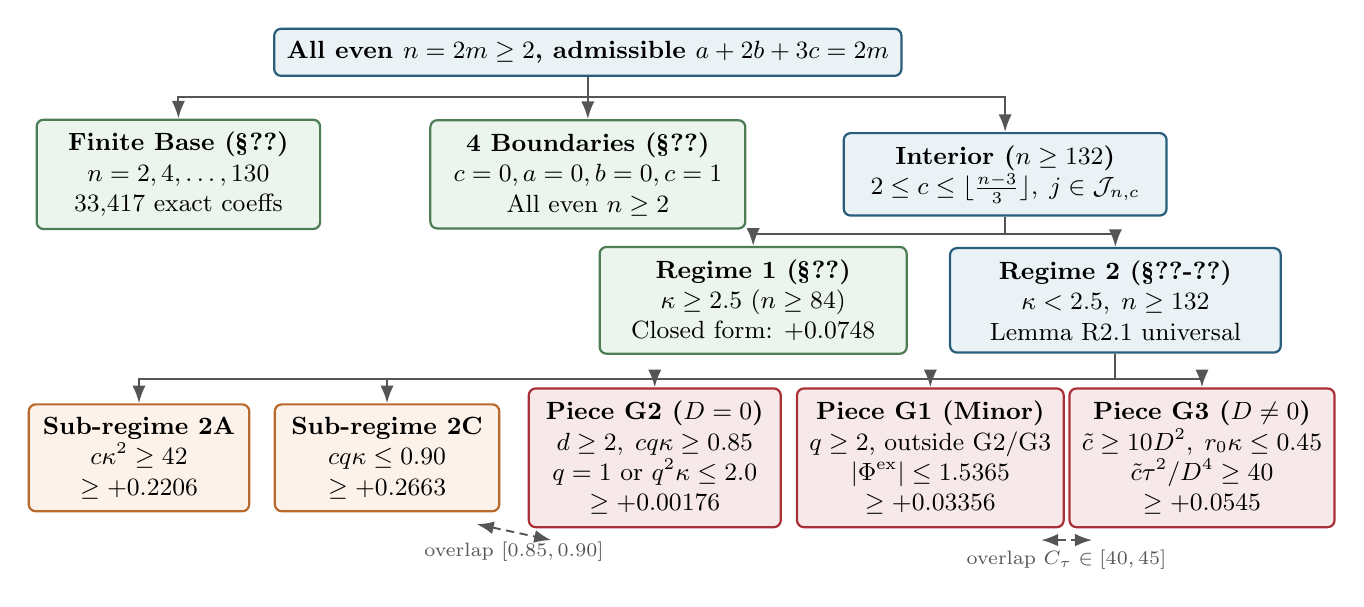
\begin{tikzpicture}[
    >=Latex,
    font=\small,
    box/.style={draw=#1, fill=#1Fill, rounded corners=2.5pt, line width=0.8pt, align=center, inner sep=4.5pt},
    arr/.style={->, line width=0.75pt, color=pGray}
]
% Top root node
\node[box=pBlue, minimum width=6.8cm] (all) at (0, 4.6)
    {\textbf{All even $n = 2m \ge 2$, admissible $a + 2b + 3c = 2m$}};

% Level 1: Base, Boundaries, Interior
\node[box=pGreen, minimum width=3.6cm] (base) at (-5.2, 3.05)
    {\textbf{Finite Base (\S\ref{sec:base})}\\$n = 2, 4, \dots, 130$\\$33{,}417$ exact coeffs};
\node[box=pGreen, minimum width=4.0cm] (bdy) at (0, 3.05)
    {\textbf{4 Boundaries (\S\ref{sec:boundaries})}\\$c=0, a=0, b=0, c=1$\\All even $n \ge 2$};
\node[box=pBlue, minimum width=4.1cm] (int) at (5.3, 3.05)
    {\textbf{Interior ($n \ge 132$)}\\$2 \le c \le \lfloor\frac{n-3}{3}\rfloor,\; j \in \mathcal{J}_{n,c}$};

\draw[arr] (all.south) -- ++(0,-0.25) -| (base.north);
\draw[arr] (all.south) -- (bdy.north);
\draw[arr] (all.south) -- ++(0,-0.25) -| (int.north);

% Level 2: Regime 1 vs Regime 2
\node[box=pGreen, minimum width=3.9cm] (reg1) at (2.1, 1.45)
    {\textbf{Regime~1 (\S\ref{sec:regime1})}\\$\kappa \ge 2.5$ ($n \ge 84$)\\Closed form: $+0.0748$};
\node[box=pBlue, minimum width=4.2cm] (reg2) at (6.7, 1.45)
    {\textbf{Regime~2 (\S\ref{sec:regime2}-\ref{sec:G3})}\\$\kappa < 2.5,\; n \ge 132$\\Lemma~R2.1 universal};

\draw[arr] (int.south) -- ++(0,-0.22) -| (reg1.north);
\draw[arr] (int.south) -- ++(0,-0.22) -| (reg2.north);

% Level 3: 5 Regime 2 Sub-regimes
\node[box=pOrange, minimum width=2.8cm] (r2a) at (-5.7, -0.55)
    {\textbf{Sub-regime 2A}\\$c\kappa^2 \ge 42$\\$\ge +0.2206$};
\node[box=pOrange, minimum width=2.85cm] (r2c) at (-2.55, -0.55)
    {\textbf{Sub-regime 2C}\\$c q \kappa \le 0.90$\\$\ge +0.2663$};
\node[box=pRed, minimum width=3.2cm] (g2) at (0.85, -0.55)
    {\textbf{Piece G2 ($D=0$)}\\$d \ge 2,\; cq\kappa \ge 0.85$\\$q=1$ or $q^2\kappa \le 2.0$\\$\ge +0.00176$};
\node[box=pRed, minimum width=3.05cm] (g1) at (4.35, -0.55)
    {\textbf{Piece G1 (Minor)}\\$q \ge 2$, outside G2/G3\\$|\Phi^{\mathrm{ex}}| \le 1.5365$\\$\ge +0.03356$};
\node[box=pRed, minimum width=3.1cm] (g3) at (7.8, -0.55)
    {\textbf{Piece G3 ($D \ne 0$)}\\$\tilde{c}\ge 10D^2,\; r_0\kappa\le 0.45$\\$\tilde{c}\tau^2/D^4 \ge 40$\\$\ge +0.0545$};

\draw[arr] (reg2.south) -- ++(0,-0.32) -| (r2a.north);
\draw[arr] (reg2.south) -- ++(0,-0.32) -| (r2c.north);
\draw[arr] (reg2.south) -- ++(0,-0.32) -| (g2.north);
\draw[arr] (reg2.south) -- ++(0,-0.32) -| (g1.north);
\draw[arr] (reg2.south) -- ++(0,-0.32) -| (g3.north);

% Overlap brackets at bottom
\draw[<->, densely dashed, pGray, line width=0.7pt]
    ($(r2c.south east)+(-0.3,-0.15)$) -- node[below, font=\scriptsize]{overlap $[0.85, 0.90]$} ($(g2.south west)+(0.3,-0.15)$);
\draw[<->, densely dashed, pGray, line width=0.7pt]
    ($(g1.south east)+(-0.3,-0.15)$) -- node[below, font=\scriptsize]{overlap $C_\tau \in [40, 45]$} ($(g3.south west)+(0.3,-0.15)$);
\end{tikzpicture}%
}
\caption{Global proof architecture and zero-crevice partition of all even integers $n = 2m \ge 2$ and admissible triples $(a, b, c)$. Green blocks denote pure exact integer or closed-form elementary proofs; amber and crimson blocks denote $50$-digit outward-rounded interval-arithmetic (\code{mpmath.iv}) proofs with strict seam overlaps.}
\label{fig:partition}
\end{figure}

\begin{proposition}[Zero-crevice partition completeness]\label{prop:zero-crevice}
Every even integer $n = 2m \ge 2$ and every admissible triple $(a, b, c) \in \Z_{\ge 0}^3$ with $a + 2b + 3c = 2m$ is covered by at least one component of Table~\ref{tab:partition}, with strict seam overlaps and zero crevices.
\end{proposition}

\begin{proof}
We verify each boundary separating adjacent regions in turn:
\begin{enumerate}[label=(\arabic*)]
    \item \emph{Degree and boundary seams:} Theorem~\ref{thm:base} covers all even $n \le 130$. For $n \ge 132$, Theorems~\ref{thm:bdy-c0} through~\ref{thm:bdy-c1} cover $c = 0$, $a = 0$, $b = 0$, and $c = 1$, which also absorbs every $c > \lfloor (n - 3)/3 \rfloor$ because $n - 3c \in \{0, 1, 2\}$ forces either $a = 0$ or $b = 0$.
    \item \emph{The $\kappa$-seam and $c\kappa^2$-seam:} For $n \ge 132$, $2 \le c \le \lfloor (n - 3)/3 \rfloor$, and $j \in \mathcal{J}_{n,c}$, Regime~1 ($\kappa \ge 2.5$, Theorem~\ref{thm:regime1}) and Regime~2 ($\kappa < 2.5$) are exact complements. Inside Regime~2, Sub-regime~2A ($c\kappa^2 \ge 42$, Theorem~\ref{thm:R2-2A}) and $\{c\kappa^2 < 42\}$ are likewise exact complements.
    \item \emph{The $c q \kappa$-seam and trichotomy inside $\{c\kappa^2 < 42,\; c q \kappa > 0.90\}$:} Sub-regime~2C-Upgrade (Theorem~\ref{thm:R2-2C}) covers $c q \kappa \le 0.90$. For any remaining point (which satisfies $c q \kappa > 0.90 > 0.88 > 0.85$, $c\kappa^2 < 42$, and $\kappa < 2.5$), let $d = \gcd(c, j) \ge 1$, $q = c/d \ge 1$, and $X = q^2\kappa$:
    \begin{itemize}[leftmargin=1.5em]
        \item \emph{Case (i): $q = 1$.} Here $d = c \ge 2$, $c q \kappa > 0.85$, and $\kappa < 2.5 = K_{\mathrm{G2}, q=1}$, so the point belongs to \textbf{Piece~G2} (Theorem~\ref{thm:G2}).
        \item \emph{Case (ii): $q \ge 2$, $d \ge 2$, and $X \le 2.0$.} Here $d \ge 2$, $q^2\kappa \le 2.0 = K_{\mathrm{G2}}$, and $c q \kappa > 0.85$, placing the point inside \textbf{Piece~G2} (Theorem~\ref{thm:G2}).
        \item \emph{Case (iii): $q \ge 2$, with either $d = 1$ (where $X = c q \kappa > 0.90 > 0.88$) or ($d \ge 2$ and $X > 2.0$).} Either there exists a coprime pair $(p_0, r_0)$ with $D := r_0 j - c p_0 \ne 0$ satisfying all four inner Piece~G3 conditions $\tilde{c} := c/r_0 \ge 10 D^2$, $r_0\kappa \le 0.45$, $r_0^3 c\kappa^2 \le 60$, and $\tilde{c}\tau^2/D^4 \ge 45 > 40$ ($\tau := c r_0 \kappa$), which places the point strictly inside \textbf{Piece~G3} (Theorem~\ref{thm:G3}, with seam overlap $[40, 45]$); or else no such $(p_0, r_0)$ exists, which places the point directly in \textbf{Piece~G1} (Theorem~\ref{thm:G1}).
    \end{itemize}
\end{enumerate}
As an independent sanity check, an exhaustive scan across all $3{,}012$ Regime~2 points for $n \in \{132, 134, \dots, 300\}$ confirms zero uncovered points.
\end{proof}

\begin{table}[htbp]
\centering
\caption{Master Zero-Crevice Partition of All Even $n = 2m \ge 2$ and Independently Certified Margins.}
\label{tab:partition}
\footnotesize
\begin{tabularx}{\textwidth}{@{} >{\raggedright\arraybackslash}p{2.35cm} >{\raggedright\arraybackslash}X >{\raggedright\arraybackslash}p{3.45cm} >{\raggedright\arraybackslash}p{2.65cm} @{}}
\toprule
\textbf{Component} & \textbf{Exact Parameter Domain} & \textbf{Proof / Arithmetic Method} & \textbf{Certified Margin} \\
\midrule
Finite Base (\S\ref{sec:base}) & Even $n = 2, 4, \dots, 130$; all $33{,}417$ coeffs & Exact integer Newton + Kronecker + $S_3$ symmetry & $0$ zeros, $0$ sign violations \\
\addlinespace[2pt]
Boundaries (\S\ref{sec:boundaries}) & All even $n \ge 2$; $c=0, a=0, b=0, c=1$ & Resultants, trig differentiation, Rolle, Maclaurin & Exact closed form \\
\addlinespace[2pt]
Regime~1 (\S\ref{sec:regime1}) & $n \ge 84$, interior, $\kappa \ge 2.5$ & Closed-form 6-subcase elementary bounds (0 search) & $+0.4699$ ($\kappa \ge 3$), $+0.0748$ ($\kappa \ge 2.5$) \\
\addlinespace[2pt]
Lemma~R2.1 (\S\ref{sec:R2-1}) & Regime~2 ($\kappa < 2.5$, $n \ge 132$) & $50$-dps \code{mpmath.iv} (0 loops) & $R_z/R_y \le e^{-37.848/\kappa}$, $c_{\mathrm{se}} \ge 3.1679$ \\
\addlinespace[2pt]
Sub-regime~2A (\S\ref{sec:R2-1}) & Regime~2, $c\kappa^2 \ge 42$ & Exact mirror-root pairing, $50$-dps \code{iv} & $\ge +0.220613$ \\
\addlinespace[2pt]
Sub-regime~2C (\S\ref{sec:R2-2C}) & Regime~2, $c q \kappa \le 0.90$ & P\'olya-Szeg\H{o} + KL harmonics, $50$-dps \code{iv} & $+0.441480$ ($q=1$), $+0.266331$ ($q\ge 2$) \\
\addlinespace[2pt]
Piece~G2 (\S\ref{sec:G2}) & $c\kappa^2 < 42$, $c q \kappa \ge 0.85$, $d \ge 2$; $\kappa < 2.5$ ($q=1$) or $q^2\kappa \le 2.0$ ($q \ge 2$) & $\pi$-line residue + Cauchy-Riemann + Euler-Maclaurin, $50$-dps \code{iv} & $+0.216651$ ($q=1$), $+0.00176348$ ($q \ge 2$) \\
\addlinespace[2pt]
Piece~G1 (\S\ref{sec:G1}) & $c\kappa^2 < 42$, $q \ge 2$, $X \ge 0.88$ ($d=1$) or $X \ge 2.0$ ($d \ge 2$), outside G3 ($C_\tau = 45$) & HS duality + CF Fibonacci ladder + $D_r^2$-cancellation, $50$-dps \code{iv} & $\ge +0.03355852$ ($|\Phi^{\mathrm{ex}}| \le 1.53645$) \\
\addlinespace[2pt]
Piece~G3 (\S\ref{sec:G3}) & $c\kappa^2 < 42$, $r_0 j = c p_0 + D$ ($D \ne 0$), $\tilde{c} \ge 10 D^2$, $r_0\kappa \le 0.45$, $r_0^3 c\kappa^2 \le 60$, $\tilde{c}\tau^2/D^4 \ge 40$ & $(1-w)$-free IBP + shifted-line 4-pole Poisson + 37 $\tau$-slices, $50$-dps \code{iv} & $\ge +0.0545$ (A1-A2, B, C, D1-D3) \\
\bottomrule
\end{tabularx}
\end{table}

The remainder of the paper is organized as follows. Section~\ref{sec:base} recalls the classical algebraic characterizations of $p_n$ and proves Theorem~\ref{thm:base} for all even $n \le 130$ via exact integer arithmetic. Section~\ref{sec:boundaries} establishes our Depressed-Cubic and Half-Size Lucas-Chebyshev resultants and delivers exact all-even-$n$ proofs for all four boundary families ($c = 0$, $a = 0$, $b = 0$, and $c = 1$). Section~\ref{sec:regime1} constructs the universal sample points $u_j$, derives the exact four-factor one-dimensional Cauchy circle integral, and proves Regime~1 ($\kappa \ge 2.5, n \ge 84$) completely in closed form. Section~\ref{sec:regime2} develops the universal Regime~2 perturbation bounds and certifies Sub-regime~2A, Sub-regime~2C-Upgrade, Piece~G2 ($D = 0$ major arcs), and Piece~G1 (Dirichlet minor arcs). Section~\ref{sec:G3} introduces the $(1-w)$-free integration-by-parts calculus and shifted-line four-pole Poisson machinery for Piece~G3 ($D \ne 0$ major arcs), and assembles the complete proof of Theorem~\ref{thm:main} and Corollary~\ref{cor:bk33}. Detailed derivations of the Regime~1 and Regime~2 auxiliary lemmas are gathered in Appendices~\ref{app:regime1} and~\ref{app:regime2}, while Appendix~\ref{app:repro} records the adversarial audit ledger, the $17$ defects uncovered and repaired prior to sign-off, and the locked SHA-256 checksums for full independent reproduction.

% ============================================================================
\section{Finite exact integer base (\texorpdfstring{$n = 2, 4, \dots, 130$}{n = 2, 4, ..., 130})}
\label{sec:base}
% ============================================================================

Before turning to asymptotic and analytic methods for arbitrarily large $n$, we first clear all small and moderate even degrees through $n = 130$ using pure integer arithmetic. Beside the defining double product~\eqref{eq:pn-def}, the Buchstaber-Novikov polynomial $p_n(x, y, z)$ admits three classical algebraic characterizations~\cite{BK2023,GRvS2024,BKor2025}:
\begin{subequations}\label{eq:classical-reps}
\begin{align}
p_n(x, y, t^n) &= \Res_u\!\bigl(u^n - x,\; (t + u)^n - (-1)^n y\bigr), \label{eq:rep-res} \\
p_n(w^n, x, y) &= \det\mathrm{Circ}_y\!\left(w^n + (-1)^{n+1} x + y,\; \binom{n}{1}w,\; \binom{n}{2}w^2,\; \dots,\; \binom{n}{n-1}w^{n-1}\right), \label{eq:rep-wendt} \\
(-1)^n (n - 1)^{2n - 2} (xyz)^{n - 2}\, p_n(x, y, z) &= \disc_T\!\Bigl(\bigl((-1)^n x T^{n-1} + (-1)^n y\bigr)(1 + T)^{n-1} - T^{n-1} z\Bigr). \label{eq:rep-disc}
\end{align}
\end{subequations}
While these identities are illuminating theoretically, computing exact integer coefficients $c_{a,b,c}^{(n)}$ all the way up to $n = 130$ is far more efficient via Newton's power sums, which remain inside exact arbitrary-precision integer arithmetic from start to finish.

\begin{theorem}[Exact integer certification for $n \le 130$]\label{thm:base}
For every even integer $n \in \{2, 4, \dots, 130\}$ ($65$ even degrees) and every admissible triple $(a, b, c) \in \Z_{\ge 0}^3$ with $a + 2b + 3c = n$, the exact integer coefficient $c_{a,b,c}^{(n)}$ is nonzero and satisfies $\sgn(c_{a,b,c}^{(n)}) = (-1)^{b(c+1)+c}$.
\end{theorem}

\begin{proof}
Treat $p_n(x, y, z) = \sum_{j=0}^{n} (-1)^j E_j(x, y) z^{n-j}$ as a monic degree-$n$ polynomial in $z$ with roots $r_k = (\alpha + \zeta^k\beta)^n$ ($0 \le k \le n - 1$). Expanding $r_k^r = \sum_{s=0}^{nr} \binom{nr}{s} \alpha^{nr-s}\beta^s \zeta^{ks}$ and summing over $k$ kills every term whose index $s$ is not a multiple of $n$, giving the exact Newton power sums
\begin{equation}\label{eq:newton-Sr}
S_r(x, y) := \sum_{k=0}^{n-1} r_k^r = n \sum_{a=0}^{r} \binom{nr}{na} x^{r-a} y^a \qquad (n \text{ even},\; 1 \le r \le n).
\end{equation}
Starting from $S_1, \dots, S_n$, Newton's identities $r E_r = \sum_{i=1}^{r} (-1)^{i-1} E_{r-i} S_i$ compute the homogeneous integer polynomials $E_r(x, y)$ exactly (\code{verify/engine.py}). Writing $s_1 = x + y$ and $s_2 = xy$ (so $e_1 = s_1 + z$, $e_2 = s_2 + s_1 z$, and $e_3 = s_2 z$), we convert from the $(s_1, s_2, z)$-basis to the $(e_1, e_2, e_3)$-basis by exact peeling in $c = 0, 1, \dots, \lfloor n/3 \rfloor$: setting $z = 0$ immediately exposes $Q_c^{(n)}(s_1, s_2)$, subtracting $Q_c^{(n)}(s_1 + z, s_2 + s_1 z)$ requires only exact integer additions, and dividing by $e_3 = s_2 z$ leaves an exact zero remainder.

For the larger degrees $n \in \{86, 88, \dots, 130\}$, \code{verify/fast\_certify\_140.py} accelerates this exact pipeline in two ways. First, $S_3$-symmetry implies that every partition $k_1 \ge k_2 \ge k_3$ with $k_1 + k_2 + k_3 = n$ obeys $k_2 + k_3 \le \lfloor 2n/3 \rfloor$, so computing only $E_0, \dots, E_{\lfloor 2n/3 \rfloor}$ uniquely determines all of $p_n$ while providing built-in symmetry cross-checks on every overlapping monomial. Second, polynomial multiplications inside Newton's recurrence are executed via exact divide-and-conquer Kronecker substitution in balanced base-$2^B$ integer encoding, with explicit assertions verifying zero carry overflow at every step.

Independent cross-checks establish three facts:
\begin{enumerate}[label=(\roman*)]
    \item \code{verify/engine.py} matches~\eqref{eq:rep-res} symbolically in SymPy for $n \le 8$ and agrees identically with the Wendt determinant~\eqref{eq:rep-wendt} for $n \le 6$;
    \item \code{verify/fast\_certify\_140.py} matches \code{verify/engine.py} bit-for-bit across every even $n \in \{2, 4, \dots, 30\}$;
    \item across $n = 2, 4, \dots, 84$ ($42$ even degrees, $9{,}464$ coefficients) and $n = 86, 88, \dots, 130$ ($23$ even degrees, $23{,}953$ coefficients), all $33{,}417$ exact integer coefficients are nonzero and obey~\eqref{eq:sign-law} with zero exceptions. \qedhere
\end{enumerate}
\end{proof}

% ============================================================================
\section{Exact structural resultants and all four boundary families}
\label{sec:boundaries}
% ============================================================================

Every proof of interior slice real-rootedness needs reliable sign anchors along the boundary of the Newton simplex. Here we establish two exact resultant representations of $P_{2m}(e_1, e_2, e_3)$ and use them, together with a palindromic Rolle-Maclaurin argument for $c = 1$, to resolve all four boundary families ($c = 0$, $a = 0$, $b = 0$, and $c = 1$) uniformly for every even integer $n = 2m \ge 2$.

\subsection{Two exact structural resultants}
\label{sec:resultants}

The vanishing locus $p_{2m}(x, y, z) = 0$ says precisely that some $2m$-th roots of $x, y, z$ sum to zero. Encoding those three zero-sum roots as the zeros of a depressed cubic immediately connects $P_{2m}$ to Waring's power-sum polynomials.

\begin{theorem}[Depressed-cubic resultant]\label{thm:res-cubic}
Let $t^3 - u t - v = 0$ have roots $t_1, t_2, t_3$ (so $t_1 + t_2 + t_3 = 0$), and set $\eta := v^2$, $x = t_1^{2m}$, $y = t_2^{2m}$, $z = t_3^{2m}$. Then $e_3(x, y, z) = \eta^m$, while $e_1(x, y, z) = \Pi_{2m}(u, \eta)$ and $e_2(x, y, z) = \Sigma_{2m}(u, \eta)$ are given by Waring's formulas:
\begin{subequations}\label{eq:waring-cubic}
\begin{align}
\Pi_{2m}(u, \eta) &:= \sum_{r=0}^{\lfloor m/3 \rfloor} \frac{2m}{m - r}\binom{m - r}{2r} u^{m - 3r}\eta^r, \\
\Sigma_{2m}(u, \eta) &:= \sum_{j=0}^{\lfloor 2m/3 \rfloor} (-1)^j \frac{m}{m - j}\binom{2m - 2j}{j} u^{2m - 3j}\eta^j.
\end{align}
\end{subequations}
Consequently:
\begin{itemize}[leftmargin=1.5em]
    \item If $3 \nmid m$, then $P_{2m}(e_1, e_2, \eta^m) = \Res_u\bigl(\Pi_{2m}(u, \eta) - e_1,\; \Sigma_{2m}(u, \eta) - e_2\bigr)$ with exact normalization $+1$.
    \item If $m = 3K$, then $\Pi_{6K}$ and $\Sigma_{6K}$ are polynomials in $w = u^3$, and $P_{6K}(e_1, e_2, e_3) = \prod_{\omega^3 = 1} R_K(e_1, e_2, \omega e_3^{1/3})$, where $R_K(e_1, e_2, \eta) := \Res_w\bigl(\tilde{\Pi}_{6K}(w, \eta) - e_1,\; \tilde{\Sigma}_{6K}(w, \eta) - e_2\bigr)$.
\end{itemize}
\end{theorem}

\begin{proof}
By~\eqref{eq:pn-def} and the identity $-1 = \zeta^m$, we have $p_{2m}(x, y, z) = 0$ if and only if $t_1 + t_2 + t_3 = 0$ for some $2m$-th roots $t_1, t_2, t_3$ of $x, y, z$. Any such triple forms the root set of a depressed cubic $t^3 - u t - v = 0$ with $v^{2m} = xyz = e_3$ and $u = -(t_1 t_2 + t_2 t_3 + t_3 t_1)$. Waring's power-sum formulas for $t_1^{2m} + t_2^{2m} + t_3^{2m}$ and $(t_1 t_2)^{2m} + (t_2 t_3)^{2m} + (t_3 t_1)^{2m}$ give~\eqref{eq:waring-cubic}. Eliminating $u$ yields a polynomial vanishing identically on the hypersurface $P_{2m}(e_1, e_2, \eta^m) = 0$. Comparing total degrees and specializing to $\eta = 0$ (where $\Pi_{2m}(u, 0) = 2u^m$ and $\Sigma_{2m}(u, 0) = u^{2m}$, giving $\Res_u(2u^m - e_1, u^{2m} - e_2) = (e_1^2 - 4e_2)^m$ when $3 \nmid m$) fixes the leading normalization to $+1$. When $m = 3K$, every power of $u$ in~\eqref{eq:waring-cubic} is divisible by $3$, giving the stated cube-root factorization.
\end{proof}

Normalizing one coordinate to $z = 1$ collapses the depressed-cubic elimination into a half-size resultant governed by Lucas-Chebyshev polynomials, which turns the $a = 0$ and $b = 0$ edges into elementary one-variable trigonometric root-counting problems.

\begin{theorem}[Half-size Lucas-Chebyshev resultant]\label{thm:res-lucas}
For each integer $n \ge 1$, define the Lucas-Chebyshev polynomial
\begin{equation}\label{eq:Ln-def}
L_n(u) := \sum_{r=0}^{\lfloor n/2 \rfloor} (-1)^r \frac{n}{n - r}\binom{n - r}{r} u^r,
\end{equation}
which obeys the algebraic identity $L_n(t(1 - t)) = t^n + (1 - t)^n$. Then for every even integer $n = 2m \ge 2$ and all $p, q \in \C$,
\begin{equation}\label{eq:lucas-res}
P_{2m}(1 + q - p,\, q,\, p)
= \Res_u\!\bigl(L_{2m}(u) + u^{2m} - q,\; u^{2m} - p\bigr)
= \prod_{k=0}^{2m-1}\Bigl(L_{2m}(\zeta^k p^{1/(2m)}) + p - q\Bigr).
\end{equation}
\end{theorem}

\begin{proof}
Setting $x_1 = t$ and $x_2 = 1 - t$ gives $x_1 + x_2 = 1$ and $x_1 x_2 = t(1 - t) = u$, so Waring's formula yields $x_1^n + x_2^n = L_n(u)$. Now fix $z = 1$ on the hypersurface $p_{2m}(x, y, z) = 0$ and write $x^{1/(2m)} = -t$ and $y^{1/(2m)} = -(1 - t)$ with $u := t(1 - t)$. Then $x + y = t^{2m} + (1 - t)^{2m} = L_{2m}(u)$ and $xy = u^{2m}$, so
\[
e_3 = u^{2m} =: p, \qquad e_2 = L_{2m}(u) + u^{2m} =: q, \qquad e_1 = 1 + q - p.
\]
Over the $2m$ roots $u_k = \zeta^k p^{1/(2m)}$ of the monic polynomial $u^{2m} - p = 0$, the product $\prod_{k=0}^{2m-1}(L_{2m}(u_k) + p - q)$ equals $\Res_u(L_{2m}(u) + u^{2m} - q,\, u^{2m} - p)$ and vanishes identically on $P_{2m}(1 + q - p, q, p) = 0$. Both sides have degree $2m$ in $q$, and at $p = 0$ (where $L_{2m}(0) = 1$) the right-hand side reduces to $(1 - q)^{2m}$, matching $P_{2m}(1 + q, q, 0) = ((1+q)^2 - 4q)^m = (1 - q)^{2m}$ from Theorem~\ref{thm:bdy-c0}. Thus~\eqref{eq:lucas-res} holds identically.
\end{proof}

\subsection{Boundary families \texorpdfstring{$c = 0$, $a = 0$, and $b = 0$}{c = 0, a = 0, and b = 0}}
\label{sec:bdy-cab}

\begin{theorem}[Boundary family $c = 0$]\label{thm:bdy-c0}
For every even integer $n = 2m \ge 2$, $Q_0^{(2m)}(e_1, e_2) = (e_1^2 - 4e_2)^m$; hence $c_{2m-2b, b, 0}^{(2m)} = (-4)^b\binom{m}{b}$ has exact sign $(-1)^b$ for all $0 \le b \le m$.
\end{theorem}

\begin{proof}
Setting $z = 0$ ($e_3 = 0$, $e_1 = x + y$, $e_2 = xy$) in~\eqref{eq:pn-def} immediately yields
\begin{align*}
p_{2m}(x, y, 0) &= \prod_{k=0}^{2m-1}\bigl(-(\alpha + \zeta^k\beta)^{2m}\bigr)
= \Bigl(\prod_{k=0}^{2m-1}(\alpha + \zeta^k\beta)\Bigr)^{2m} \\
&= (\alpha^{2m} - \beta^{2m})^{2m} = (x - y)^{2m} = (e_1^2 - 4e_2)^m. \qedhere
\end{align*}
\end{proof}

\begin{theorem}[Boundary families $a = 0$ and $b = 0$]\label{thm:bdy-ab}
For every even integer $n = 2m \ge 2$:
\begin{enumerate}[label=\textup{(\arabic*)}]
    \item The univariate polynomial $f_a^{(2m)}(w) := \sum_{q=0}^{\lfloor m/3 \rfloor} c_{0,\, m-3q,\, 2q}^{(2m)}\, w^q$ has $\lfloor m/3 \rfloor$ simple strictly positive real roots in $w = e_3^2/e_2^3 \in (0, +\infty)$, and $\sgn(c_{0, m-3q, 2q}^{(2m)}) = (-1)^{m-q}$ for all $0 \le q \le \lfloor m/3 \rfloor$.
    \item The univariate polynomial $f_b^{(2m)}(w) := \sum_{c=0}^{\lfloor 2m/3 \rfloor} c_{2m-3c,\, 0,\, c}^{(2m)}\, w^c$ has $\lfloor 2m/3 \rfloor$ simple strictly positive real roots in $w = e_3/e_1^3 \in (0, +\infty)$, and $\sgn(c_{2m-3c, 0, c}^{(2m)}) = (-1)^c$ for all $0 \le c \le \lfloor 2m/3 \rfloor$.
\end{enumerate}
\end{theorem}

\begin{proof}
Parameterize $u \in [1/4, +\infty)$ by $u = \frac{1}{4\cos^2\theta}$ with $\theta \in [0, \pi/2)$. Since $t = \frac{e^{i\theta}}{2\cos\theta}$ obeys $1 - t = \frac{e^{-i\theta}}{2\cos\theta}$ and $t(1 - t) = u$, the defining identity of $L_{2m}$ yields
\begin{subequations}\label{eq:L-trig}
\begin{align}
L_{2m}\!\Bigl(\frac{1}{4\cos^2\theta}\Bigr) &= \frac{2\cos(2m\theta)}{(2\cos\theta)^{2m}}, \label{eq:L-trig-a} \\
\frac{\dd}{\dd\theta}\!\left[\frac{2\cos(2m\theta)}{(2\cos\theta)^{2m}}\right] &= \frac{-8m\sin((2m - 1)\theta)}{(2\cos\theta)^{2m+1}}, \label{eq:L-trig-b} \\
\frac{\dd}{\dd\theta}\!\Bigl[2(2\cos\theta)^{2m}\cos(2m\theta) + 1\Bigr] &= -8m(2\cos\theta)^{2m-1}\sin((2m + 1)\theta). \label{eq:L-trig-c}
\end{align}
\end{subequations}

\emph{Part~(1) ($a = 0$, i.e.\ $e_1 = 0$).} Setting $q = p - 1$ in Theorem~\ref{thm:res-lucas} gives
\[
(p - 1)^m f_a^{(2m)}\!\Bigl(\frac{p^2}{(p - 1)^3}\Bigr) = P_{2m}(0, p - 1, p) = \Res_u(L_{2m}(u) + 1,\, u^{2m} - p).
\]
Every root $u_* \in (1, +\infty)$ of $L_{2m}(u) + 1 = 0$ produces $p_* = u_*^{2m} \in (1, +\infty)$ and a positive root $w_* = \frac{p_*^2}{(p_* - 1)^3}$ of $f_a^{(2m)}$. Because $\frac{\dd}{\dd p}\frac{p^2}{(p-1)^3} = -\frac{p(p+2)}{(p-1)^4} < 0$ on $(1, +\infty)$, distinct roots $u_* > 1$ map injectively to distinct positive roots $w_*$.

Consider $h_a(\theta) := L_{2m}(\frac{1}{4\cos^2\theta}) + 1 = \frac{2\cos(2m\theta)}{(2\cos\theta)^{2m}} + 1$ on $(\pi/3, \pi/2)$ (where $2\cos\theta \in (0, 1)$, so $u > 1$). Put $r_{\min} := m - \lfloor m/3 \rfloor$ and evaluate $h_a$ at the critical points $\theta_r := \frac{r\pi}{2m - 1}$ ($r = r_{\min}, \dots, m - 1$) identified by~\eqref{eq:L-trig-b}. Since $3 r_{\min} \ge 2m > 2m - 1$, every $\theta_r$ lies in $(\pi/3, \pi/2)$, so $(2\cos\theta_r)^{1-2m} > 1$. Writing $2m\theta_r = r\pi + \theta_r$ gives $\cos(2m\theta_r) = (-1)^r\cos\theta_r$, whence
\[
h_a(\theta_r) = 1 + (-1)^r (2\cos\theta_r)^{1-2m}, \qquad \sgn(h_a(\theta_r)) = (-1)^r \qquad (r = r_{\min}, \dots, m - 1).
\]
As $\theta \to (\pi/2)^-$, $h_a(\theta) \sim 2(-1)^m(2\cos\theta)^{-2m}$ carries sign $(-1)^m$. Across the $\lfloor m/3 \rfloor + 1$ ordered points $\theta_{r_{\min}} < \dots < \theta_{m-1} < (\pi/2)^-$, $h_a$ strictly alternates sign $\lfloor m/3 \rfloor$ times, isolating all $\lfloor m/3 \rfloor$ simple positive roots of $f_a^{(2m)}(w)$. Since $f_a^{(2m)}(0) = c_{0, m, 0}^{(2m)} = (-4)^m$ (Theorem~\ref{thm:bdy-c0}), Vieta's formulas force $\sgn(c_{0, m-3q, 2q}^{(2m)}) = (-1)^{m-q}$.

\emph{Part~(2) ($b = 0$, i.e.\ $e_2 = 0$).} Setting $q = 0$ in Theorem~\ref{thm:res-lucas} gives
\[
(1 - p)^{2m} f_b^{(2m)}\!\Bigl(\frac{p}{(1 - p)^3}\Bigr) = P_{2m}(1 - p, 0, p) = \Res_u(L_{2m}(u) + u^{2m},\, u^{2m} - p).
\]
Every root $u_* \in (1/4, 1)$ of $L_{2m}(u) + u^{2m} = 0$ produces $p_* = u_*^{2m} \in (4^{-2m}, 1)$ and $w_* = \frac{p_*}{(1-p_*)^3} > 0$, injectively since $\frac{\dd}{\dd p}\frac{p}{(1-p)^3} = \frac{1+2p}{(1-p)^4} > 0$ on $(0, 1)$. Define $h_b(\theta) := 2(2\cos\theta)^{2m}\cos(2m\theta) + 1$ on $[0, \pi/3)$ (where $2\cos\theta \in (1, 2]$). At the critical points $\tilde{\theta}_r := \frac{r\pi}{2m + 1}$ ($r = 0, \dots, \lfloor 2m/3 \rfloor$) from~\eqref{eq:L-trig-c}, we have $\tilde{\theta}_r < \pi/3$, $(2\cos\tilde{\theta}_r)^{2m+1} > 1$, and $2m\tilde{\theta}_r = r\pi - \tilde{\theta}_r$, giving
\[
h_b(\tilde{\theta}_r) = 1 + (-1)^r (2\cos\tilde{\theta}_r)^{2m+1}, \qquad \sgn(h_b(\tilde{\theta}_r)) = (-1)^r \qquad (r = 0, \dots, \lfloor 2m/3 \rfloor).
\]
Because $h_b(0) = 2^{2m+1} + 1 > 0$, this isolates all $\lfloor 2m/3 \rfloor$ simple positive real roots of $f_b^{(2m)}(w)$, and $f_b^{(2m)}(0) = c_{2m,0,0}^{(2m)} = +1$ forces $\sgn(c_{2m-3c, 0, c}^{(2m)}) = (-1)^c$ by Vieta's formulas.
\end{proof}

\subsection{Boundary family \texorpdfstring{$c = 1$}{c = 1}}
\label{sec:bdy-c1}

The slice $c = 1$ requires a different idea, because its coefficients are uniformly negative and cannot be read off by setting $e_1 = 0$ or $e_2 = 0$. Differentiating $p_{2m}(1, u, z)$ once at $z = 0$ expresses $Q_1^{(2m)}$ in terms of an auxiliary palindromic polynomial $A_{2m-1}^{(2m)}(u)$ whose simple negative real-rootedness unlocks Maclaurin's inequality.

\begin{theorem}[Boundary family $c = 1$]\label{thm:bdy-c1}
For every even integer $n = 2m \ge 4$ and every $0 \le b \le m - 2$, we have $c_{2m-3-2b,\, b,\, 1}^{(2m)} < 0$.
\end{theorem}

\begin{proof}
Set $x = 1$ and $y = u$, and differentiate $p_n(1, u, z) = (e_1^2 - 4e_2)^m + e_3 Q_1^{(2m)}(e_1, e_2) + O(e_3^2)$ with respect to $z$ at $z = 0$ (where $e_1 = 1 + u$, $e_2 = u$, $e_3 = 0$, $\partial_z e_1 = 1$, $\partial_z e_2 = 1 + u$, and $\partial_z e_3 = u$). Matching both sides gives
\[
-2m(1 + u)(1 - u)^{2m - 2} + u\, Q_1^{(2m)}(1 + u, u) = -(1 - u)^n \sum_{k=0}^{n-1} \frac{1}{(1 + \zeta^k u^{1/n})^n} =: -2m\, A_{2m - 1}^{(2m)}(u),
\]
where for $1 \le r \le n$ we set $S_r(u) := \frac{1}{n}\sum_{k=0}^{n-1}(1 + \zeta^k u^{1/n})^{-r}$, $F_r(u) := (1 - u)^r S_r(u)$, and $A_{2m-1}^{(2m)}(u) := F_{2m}(u)$.

\emph{Step 1 (Rolle real-rootedness of $F_r$).} Since $S_1(u) = (1 - u)^{-1}$, we start with $F_1(u) = 1$. Differentiating $S_{r-1}$ term-by-term gives $S_r(u) = S_{r-1}(u) + \frac{nu}{r-1} S'_{r-1}(u)$; multiplying by $(1 - u)^r$ yields the polynomial recurrence ($2 \le r \le n$)
\begin{equation}\label{eq:Fr-rec}
(r - 1)\, F_r(u) = n u(1 - u)\, F'_{r-1}(u) + (r - 1)\bigl(1 + (n - 1)u\bigr)\, F_{r-1}(u).
\end{equation}
We verify by induction on $r \in \{1, \dots, n\}$ that $F_r(u)$ has exact degree $r - 1$, satisfies $F_r(0) = 1$, has positive leading coefficient $\binom{n-1}{r-1}$, and possesses $r - 1$ simple strictly negative real roots. Indeed, at the $r - 2$ simple negative roots $\xi_1 < \dots < \xi_{r-2} < 0$ of $F_{r-1}$, the prefactor $n\xi_j(1 - \xi_j)$ is strictly negative while $F'_{r-1}(\xi_j)$ alternates sign, forcing strict sign alternation of $F_r(\xi_j)$. Since $F_r(0) = 1 > 0$ and $F'_{r-1}(\xi_{r-2}) > 0$ implies $F_r(\xi_{r-2}) < 0$, the polynomial $F_r$ acquires a root in $(\xi_{r-2}, 0)$, $r - 3$ roots between consecutive $\xi_j$, and one further root in $(-\infty, \xi_1)$ by positivity of its leading coefficient.

\emph{Step 2 (Palindromic factorization and exact coefficient formula).} At $r = n = 2m$, the inversion $u \mapsto u^{-1}$ merely permutes the summands of $S_{2m}$, showing that $A_{2m-1}^{(2m)}(u)$ is monic, palindromic ($A_{2m-1}^{(2m)}(u^{-1}) = u^{-(2m-1)} A_{2m-1}^{(2m)}(u)$), of odd degree $2m - 1$, with $2m - 1$ simple strictly negative real roots. Consequently $u = -1$ is a root and the remaining roots come in reciprocal pairs $(r_j, r_j^{-1})$ with $r_j < -1$ ($1 \le j \le m - 1$). Putting $c_j := -(r_j + r_j^{-1}) - 2 = (\sqrt{-r_j} - 1/\sqrt{-r_j})^2 > 0$ and $\gamma_r := e_r(c_1, \dots, c_{m-1}) > 0$ ($\gamma_0 = 1$), we obtain
\[
\frac{A_{2m-1}^{(2m)}(u)}{1 + u} = \prod_{j=1}^{m-1}\bigl((1 + u)^2 + c_j u\bigr) = \sum_{r=0}^{m-1} \gamma_r (1 + u)^{2m - 2 - 2r} u^r.
\]
Comparing this with $(1 - u)^{2m-2} = ((1 + u)^2 - 4u)^{m-1} = \sum_{r=0}^{m-1} (-4)^r \binom{m-1}{r}(1 + u)^{2m-2-2r} u^r$, the $r = 0$ terms cancel identically in $u\, Q_1^{(2m)}(1 + u, u) = 2m\bigl((1 + u)(1 - u)^{2m - 2} - A_{2m-1}^{(2m)}(u)\bigr)$, leaving the exact identity
\begin{equation}\label{eq:c1-exact}
c_{2m - 3 - 2b,\, b,\, 1}^{(2m)} = 2m\Bigl((-4)^{b+1}\binom{m - 1}{b + 1} - \gamma_{b+1}\Bigr) \qquad (0 \le b \le m - 2).
\end{equation}

\emph{Step 3 (Maclaurin's inequality and an alternating trigonometric sum).} Because $c_1, \dots, c_{m-1} > 0$, Maclaurin's inequality~\cite{HLP1952} yields $\bigl(\gamma_r / \binom{m-1}{r}\bigr)^{1/r} \ge \gamma_{m-1}^{1/(m-1)}$ for every $1 \le r \le m - 1$. Therefore, showing $\gamma_{m-1} > 4^{m-1}$ immediately forces $\gamma_r > 4^r\binom{m-1}{r}$ for every $r$, and hence $c_{2m-3-2b, b, 1}^{(2m)} < 0$ for every $b$. Evaluating $\frac{A_{2m-1}^{(2m)}(u)}{1 + u}$ at $u = -1$ via L'H\^opital's rule gives $\gamma_{m-1} = (-1)^{m-1}(A_{2m-1}^{(2m)})'(-1)$. Using $u^{1/(2m)}\big|_{u=-1} = e^{i\pi/(2m)}$ and $1 + e^{i(2k+1)\pi/(2m)} = 2\cos\frac{(2k+1)\pi}{4m}\, e^{i(2k+1)\pi/(4m)}$, differentiating $A_{2m-1}^{(2m)}$ at $u = -1$ and pairing $k$ with $2m - 1 - k$ yields the exact alternating trigonometric sum
\begin{equation}\label{eq:gamma-trig}
\gamma_{m - 1} = \frac{1}{2m}\sum_{k=0}^{m-1} (-1)^k \frac{\cos\theta_k}{\sin^{2m+1}\theta_k}, \qquad \theta_k := \frac{(2k + 1)\pi}{4m}.
\end{equation}
Since $\theta \mapsto \frac{\cos\theta}{\sin^{2m+1}\theta}$ is strictly decreasing on $(0, \pi/2)$ and $\frac{\sin\theta_1}{\sin\theta_0} = 3 - 4\sin^2\frac{\pi}{4m} \ge 3 - 4\sin^2\frac{\pi}{8} = 1 + \sqrt{2} > 2$ for every $m \ge 2$, the alternating sum exceeds its first two terms:
\[
\gamma_{m - 1} > \frac{\cos(\pi/8)}{2m}\Bigl(\frac{4m}{\pi}\Bigr)^{2m + 1}\Bigl(1 - \frac{1}{2^{2m + 1}}\Bigr) > 4^{m - 1} \qquad (\forall m \ge 2).
\]
Explicitly, at $m = 2$ we have $\gamma_1 = 28 > 4$, while for $m \ge 3$ we have $\frac{4m}{\pi} > 3.81$, so $(\frac{4m}{\pi})^{2m} > 14.5^m \gg 4^{m-1}$.
\end{proof}

% ============================================================================
\section{Universal sample points, exact 1D circle integral, and Regime~1}
\label{sec:regime1}
% ============================================================================

Having secured the finite base ($n \le 130$) and all four boundaries (all even $n \ge 2$), we now move into the heart of the problem: the interior slices $2 \le c \le \lfloor (n - 3)/3 \rfloor$. The key conceptual breakthrough of this paper is to evaluate $Q_c^{(2m)}(1, u)$ along a carefully chosen family of trigonometric sample points $u_j$ where the associated Cauchy contour integral collapses to a one-dimensional integral with a nonnegative boundary kernel.

\subsection{Universal trigonometric sample points and root interleaving}
\label{sec:sample-points}

\begin{theorem}[Universal sample points and root-interleaving reduction]\label{thm:sample-points}
Fix even $n = 2m \ge 6$ and $2 \le c \le \lfloor (n - 3)/3 \rfloor$. Set $D_c := \lfloor (n - 3c)/2 \rfloor$ and let $\mathcal{J}_{n,c}$ be given by~\eqref{eq:Jnc}. For each $j \in \mathcal{J}_{n, c}$, define
\begin{subequations}\label{eq:sample-params}
\begin{align}
\theta_c &:= \frac{c\pi}{n}, \qquad \psi_j := \frac{j\pi}{n}, \qquad \alpha_1 := \frac{(j + c)\pi}{n}, \qquad
r_1 := \sin\alpha_1, \quad r_2 := \sin\psi_j, \quad r_3 := \sin\theta_c, \\
s_j &:= \frac{r_2}{r_1} \in (0, 1), \qquad R_y := s_j^n, \qquad R_z := \Bigl(\frac{r_3}{r_1}\Bigr)^n, \qquad
t_j := (-1)^c R_y, \qquad u_j := \frac{t_j}{(1 + t_j)^2}.
\end{align}
\end{subequations}
If $(-1)^j Q_c^{(2m)}(1, u_j) > 0$ for every $j \in \mathcal{J}_{n, c}$, then $Q_c^{(2m)}(1, u)$ has $D_c$ simple real roots, all in $(0, +\infty)$ (with at least $D_c - 1$ strictly inside $(0, 1/4)$) when $c$ is even and all in $(-\infty, 0)$ when $c$ is odd. Consequently, every coefficient $c_{n-3c-2b, b, c}^{(2m)}$ ($0 \le b \le D_c$) is nonzero with exact sign $(-1)^{b(c+1)+c}$.
\end{theorem}

\begin{figure}[htbp]
\centering
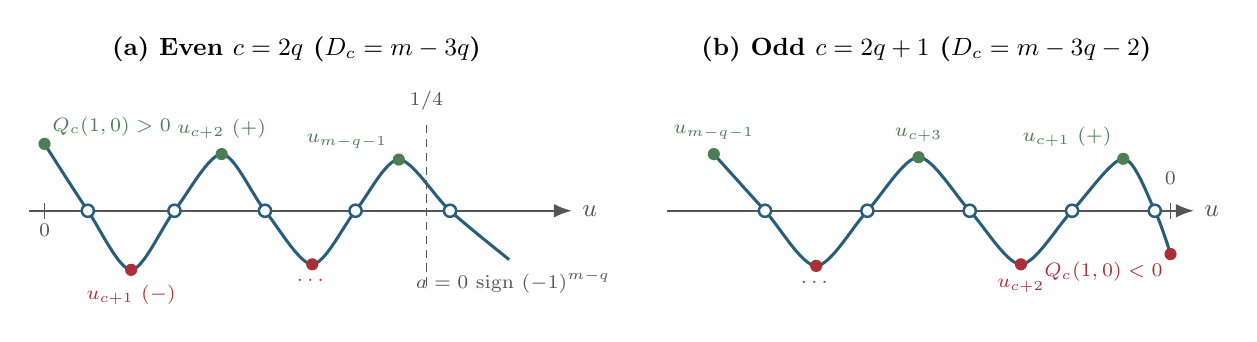
\begin{tikzpicture}[>=Latex, font=\small]
% Panel (a): Even c
\begin{scope}[xshift=0cm]
\node[font=\small\bfseries] at (3.2, 2.05) {(a) Even $c = 2q$ ($D_c = m - 3q$)};
\draw[->, line width=0.8pt, pGray] (-0.2, 0) -- (6.7, 0) node[right]{$u$};
% Oscillating curve
\draw[pBlue, line width=1.1pt, smooth]
    plot coordinates {(0,0.85) (0.55,0) (1.1,-0.75) (1.65,0) (2.25,0.72) (2.8,0) (3.4,-0.68) (3.95,0) (4.5,0.65) (5.15,0) (5.9,-0.62)};
% Tick 0 and 1/4
\draw[pGray, line width=0.7pt] (0, -0.1) -- (0, 0.1) node[below=4pt, font=\scriptsize]{$0$};
\draw[pGray, densely dashed, line width=0.6pt] (4.85, -0.95) -- (4.85, 1.15);
\node[above, font=\scriptsize, pGray] at (4.85, 1.15) {$1/4$};
% Sample points u_j
\fill[pGreen] (0,0.85) circle (2.2pt) node[above right=-1pt, font=\scriptsize]{$Q_c(1,0)>0$};
\fill[pRed] (1.1,-0.75) circle (2.2pt) node[below=2pt, font=\scriptsize]{$u_{c+1}$ ($-$)};
\fill[pGreen] (2.25,0.72) circle (2.2pt) node[above=2pt, font=\scriptsize]{$u_{c+2}$ ($+$)};
\fill[pRed] (3.4,-0.68) circle (2.2pt) node[below=2pt, font=\scriptsize]{$\dots$};
\fill[pGreen] (4.5,0.65) circle (2.2pt) node[above left=1pt, font=\scriptsize]{$u_{m-q-1}$};
% Roots
\foreach \rx in {0.55, 1.65, 2.8, 3.95, 5.15} {
    \fill[white] (\rx, 0) circle (2.2pt);
    \draw[pBlue, line width=0.9pt] (\rx, 0) circle (2.2pt);
}
\node[font=\scriptsize, pGray] at (5.95, -0.9) {$a=0$ sign $(-1)^{m-q}$};
\end{scope}

% Panel (b): Odd c
\begin{scope}[xshift=8.1cm]
\node[font=\small\bfseries] at (3.1, 2.05) {(b) Odd $c = 2q + 1$ ($D_c = m - 3q - 2$)};
\draw[->, line width=0.8pt, pGray] (-0.2, 0) -- (6.5, 0) node[right]{$u$};
\draw[pBlue, line width=1.1pt, smooth]
    plot coordinates {(0.4,0.72) (1.05,0) (1.7,-0.70) (2.35,0) (3.0,0.68) (3.65,0) (4.3,-0.68) (4.95,0) (5.6,0.66) (6.0,0) (6.2,-0.55)};
\draw[pGray, line width=0.7pt] (6.2, -0.1) -- (6.2, 0.1) node[above=3pt, font=\scriptsize]{$0$};
\fill[pRed] (6.2,-0.55) circle (2.2pt) node[below left=-1pt, font=\scriptsize]{$Q_c(1,0)<0$};
\fill[pGreen] (0.4,0.72) circle (2.2pt) node[above=2pt, font=\scriptsize]{$u_{m-q-1}$};
\fill[pRed] (1.7,-0.70) circle (2.2pt) node[below=2pt, font=\scriptsize]{$\dots$};
\fill[pGreen] (3.0,0.68) circle (2.2pt) node[above=2pt, font=\scriptsize]{$u_{c+3}$};
\fill[pRed] (4.3,-0.68) circle (2.2pt) node[below=2pt, font=\scriptsize]{$u_{c+2}$};
\fill[pGreen] (5.6,0.66) circle (2.2pt) node[above left=1pt, font=\scriptsize]{$u_{c+1}$ ($+$)};
\foreach \rx in {1.05, 2.35, 3.65, 4.95, 6.0} {
    \fill[white] (\rx, 0) circle (2.2pt);
    \draw[pBlue, line width=0.9pt] (\rx, 0) circle (2.2pt);
}
\end{scope}
\end{tikzpicture}
\caption{Universal trigonometric sample points $u_j$ strictly interleaving the $D_c$ simple real roots (open circles) of $Q_c^{(2m)}(1, u)$. (a) For even $c = 2q$, the $D_c - 1$ sample points lie in $(0, 1/4)$ and combine with $Q_c(1,0) > 0$ and the $a = 0$ leading sign $(-1)^{m-q}$ to isolate $D_c$ positive roots. (b) For odd $c = 2q+1$, the $D_c$ sample points lie in $(-\infty, 0)$ and combine with $Q_c(1,0) < 0$ to isolate $D_c$ negative roots.}
\label{fig:interleaving}
\end{figure}

\begin{proof}
For every $j \in \mathcal{J}_{n,c}$ we have $0 < j < \min(j + c, n - j - c) \le n/2$, so $s_j \in (0, 1)$. Moreover, $\frac{\dd}{\dd x}\frac{\sin x}{\sin(x + \theta_c)} = \frac{\sin\theta_c}{\sin^2(x + \theta_c)} > 0$ shows that $s_j$ increases strictly with $j$ (Figure~\ref{fig:interleaving}).
\begin{itemize}[leftmargin=1.5em]
    \item \emph{Even $c = 2q$:} Here $D_c = m - 3q$ and $|\mathcal{J}_{n, c}| = D_c - 1$. As $j$ increases, $t_j = s_j^n \in (0, 1)$ rises strictly, giving $0 < u_{c+1} < \dots < u_{m-q-1} < \frac{1}{4}$. Combining $Q_c^{(2m)}(1, 0) = c_{n-3c,0,c}^{(2m)} > 0$ (Theorem~\ref{thm:bdy-ab}), the $D_c - 1$ alternating signs $(-1)^j Q_c^{(2m)}(1, u_j) > 0$, and the leading-coefficient sign $\sgn(c_{0, m-3q, 2q}^{(2m)}) = (-1)^{m-q}$ (opposite to $(-1)^{m-q-1}$, Theorem~\ref{thm:bdy-ab}) forces $D_c$ sign changes on $(0, +\infty)$, and thus $D_c$ simple positive real roots (with at least $D_c - 1$ inside $(0, 1/4)$).
    \item \emph{Odd $c = 2q + 1$:} Here $D_c = m - 3q - 2$ and $|\mathcal{J}_{n, c}| = D_c$. As $j$ increases, $t_j = -s_j^n \in (-1, 0)$ decreases strictly, and $\frac{\dd}{\dd t}\frac{t}{(1+t)^2} = \frac{1-t}{(1+t)^3} > 0$ on $(-1, 0)$ gives $-\infty < u_{m-q-1} < \dots < u_{c+1} < 0$. Pairing these $D_c$ strictly alternating values with $Q_c^{(2m)}(1, 0) < 0$ (Theorem~\ref{thm:bdy-ab}) creates $D_c$ sign changes strictly inside $(u_{m-q-1}, 0) \subset (-\infty, 0)$, hence $D_c$ simple negative real roots.
\end{itemize}
In both parities, Vieta's formulas together with $\sgn(Q_c^{(2m)}(1, 0)) = (-1)^c$ force the universal sign law~\eqref{eq:sign-law}.
\end{proof}

\subsection{Exact four-factor 1D Cauchy circle integral}
\label{sec:circle-integral}

Why were the angles $\theta_c$, $\psi_j$, and $\alpha_1$ chosen in~\eqref{eq:sample-params}? By the Law of Sines on the triangle with angles $(\theta_c, \psi_j, \pi - \alpha_1)$ (Figure~\ref{fig:circle-geom}(a)), the two boundary roots $w_{\pm\theta_c} := (1 - s_j e^{\pm i\theta_c})^n$ land simultaneously at the exact real value $(-1)^j R_z$, while every other root separates cleanly into $|w_k| < R_z$ (small) or $|w_k| > R_z$ (large). Extracting the coefficient of $e_3^c$ by Cauchy's integral formula turns $(-1)^j Q_c^{(2m)}(1, u_j)$ into the following exact one-dimensional integral.

\begin{theorem}[Exact 4-factor 1D circle integral]\label{thm:circle-integral}
Fix even $n = 2m \ge 6$, $2 \le c \le \lfloor (n - 3)/3 \rfloor$, and $j \in \mathcal{J}_{n, c}$. For $|w| = \lambda > 0$, consider the cubic equation
\begin{equation}\label{eq:cubic}
T(T - 1)(T - t) = t R_z w \qquad \bigl(t := t_j = (-1)^c R_y\bigr).
\end{equation}
Suppose Rouch\'e's theorem isolates unique simple roots $x(w) = 1 + \delta_x(w)$ and $y(w) = t(1 + \tilde{\delta}_y(w))$ holomorphic on a neighborhood of $|w| \le \lambda$ with $|\delta_x| < 1$ and $|\delta_y| < 1$, where
\begin{equation}\label{eq:deltas}
1 + \delta_y(w) := \frac{y(w)}{t\, x(w)}, \qquad
1 + \delta_z(w) := \frac{z(w)}{x(w) R_z w} = \frac{1}{(1 + \delta_x(w))^3(1 + \delta_y(w))},
\end{equation}
and set $\varepsilon_s(w) := (1 + \delta_y(w))^{1/n} - 1$ (principal branch). Let the $n$ angles $\eta_k \in (-\pi, \pi]$ be $\frac{2k\pi}{n}$ (even $c$) or $\frac{(2k+1)\pi}{n}$ (odd $c$), partitioned into \emph{small} ($|\eta_k| < \theta_c$, count $c - 1$), \emph{boundary} ($|\eta_k| = \theta_c$, namely $\pm\theta_c$), and \emph{large} ($|\eta_k| > \theta_c$, count $n - c - 1$). Put $w_k := (1 - s_j e^{i\eta_k})^n$, $a_k^{\mathrm{alg}} := \frac{-s_j e^{i\eta_k}}{1 - s_j e^{i\eta_k}}$, $\tilde{w}_k := w_k (1 + a_k^{\mathrm{alg}}\varepsilon_s)^n$, $1 + \varepsilon_\pm(w) := (1 + a^{\mathrm{alg}}(\pm\theta_c)\varepsilon_s(w))^n$, and $Z := (-1)^j w^{-1}$. Then
\begin{equation}\label{eq:circle-integral}
(-1)^j (1 + t)^{n - 3c} Q_c^{(2m)}(1, u_j)
= \frac{C_{m,c,j}}{2\pi}\int_{-\pi}^{\pi} \bigl(1 + \Delta_{\mathrm{mult}}(\lambda e^{i\phi})\bigr)\, B(\lambda e^{i\phi})\, \dd\phi,
\qquad C_{m,c,j} := \frac{R_z \prod_{\mathrm{large}} |w_k|}{R_y^c} > 0,
\end{equation}
where $1 + \Delta_{\mathrm{mult}}(w) := F_1(w)\, F_2(w)\, F_3(w)$ and
\begin{subequations}\label{eq:F123B}
\begin{align}
F_1(w) &:= (1 + \delta_x)^{n - 3c}, \qquad
F_2(w) := \frac{\prod_{\mathrm{large}}(1 + a_k^{\mathrm{alg}} \varepsilon_s)^n}{(1 + \delta_y)^c}, \label{eq:F123B-a} \\
F_3(w) &:= \prod_{\mathrm{small}}\!\Bigl(1 - \frac{\tilde{w}_k}{z/x}\Bigr)\prod_{\mathrm{large}}\!\Bigl(1 - \frac{z/x}{\tilde{w}_k}\Bigr), \label{eq:F123B-b} \\
B(w) &:= \frac{(-Z^{-1})\bigl((1 + \delta_z) - Z(1 + \varepsilon_+)\bigr)\bigl((1 + \delta_z) - Z(1 + \varepsilon_-)\bigr)}{1 + \delta_z} \nonumber \\
&= (2 - Z - Z^{-1}) - Z^{-1}\delta_z + (\varepsilon_+ + \varepsilon_-) - Z\Bigl((1 + \varepsilon_+)(1 + \varepsilon_-)(1 + \delta_x)^3(1 + \delta_y) - 1\Bigr). \label{eq:F123B-c}
\end{align}
\end{subequations}
\end{theorem}

\begin{figure}[htbp]
\centering
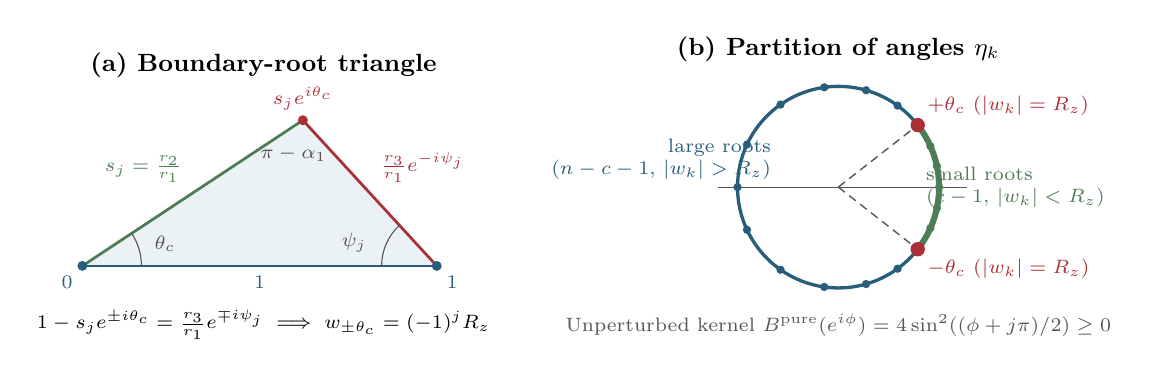
\begin{tikzpicture}[>=Latex, font=\small]
% Panel (a): Law of Sines triangle
\begin{scope}[xshift=0cm, yshift=-0.2cm]
\node[font=\small\bfseries] at (2.3, 2.55) {(a) Boundary-root triangle};
\coordinate (O) at (0, 0);
\coordinate (A) at (4.5, 0);
\coordinate (P) at (2.8, 1.85);
\fill[pBlueFill] (O) -- (A) -- (P) -- cycle;
\draw[pBlue, line width=1.0pt] (O) -- node[below, font=\scriptsize]{$1$} (A);
\draw[pGreen, line width=1.0pt] (O) -- node[above left, font=\scriptsize]{$s_j = \frac{r_2}{r_1}$} (P);
\draw[pRed, line width=1.0pt] (A) -- node[above right, font=\scriptsize]{$\frac{r_3}{r_1} e^{-i\psi_j}$} (P);
\fill[pBlue] (O) circle (1.8pt) node[below left, font=\scriptsize]{$0$};
\fill[pBlue] (A) circle (1.8pt) node[below right, font=\scriptsize]{$1$};
\fill[pRed] (P) circle (1.8pt) node[above, font=\scriptsize]{$s_j e^{i\theta_c}$};
% Angle arcs
\draw[pGray] (0.75, 0) arc (0:33.5:0.75);
\node[font=\scriptsize, pGray] at (1.05, 0.28) {$\theta_c$};
\draw[pGray] (3.8, 0) arc (180:132.5:0.7);
\node[font=\scriptsize, pGray] at (3.45, 0.30) {$\psi_j$};
\node[font=\scriptsize, pGray] at (2.68, 1.42) {$\pi-\alpha_1$};
\node[font=\scriptsize, align=center] at (2.3, -0.75) {$1 - s_j e^{\pm i\theta_c} = \frac{r_3}{r_1} e^{\mp i\psi_j} \implies w_{\pm\theta_c} = (-1)^j R_z$};
\end{scope}

% Panel (b): Unit circle root partition
\begin{scope}[xshift=9.6cm, yshift=0.8cm]
\node[font=\small\bfseries] at (0, 1.75) {(b) Partition of angles $\eta_k$};
\def\radC{1.28}
% Small arc
\draw[pGreen, line width=2.2pt] ({ \radC*cos(-38) }, { \radC*sin(-38) }) arc (-38:38:\radC);
% Large arc
\draw[pBlue, line width=1.2pt] ({ \radC*cos(38) }, { \radC*sin(38) }) arc (38:322:\radC);
% Center & rays
\draw[pGray, densely dashed, line width=0.5pt] (0,0) -- ({ \radC*cos(38) }, { \radC*sin(38) });
\draw[pGray, densely dashed, line width=0.5pt] (0,0) -- ({ \radC*cos(-38) }, { \radC*sin(-38) });
\draw[pGray, line width=0.4pt] (-\radC-0.25,0) -- (\radC+0.35,0);
% Boundary roots
\fill[pRed] ({ \radC*cos(38) }, { \radC*sin(38) }) circle (2.6pt) node[above right, font=\scriptsize, pRed]{$+\theta_c$ ($|w_k|=R_z$)};
\fill[pRed] ({ \radC*cos(-38) }, { \radC*sin(-38) }) circle (2.6pt) node[below right, font=\scriptsize, pRed]{$-\theta_c$ ($|w_k|=R_z$)};
% Sample dots
\foreach \ang in {-24,-12,0,12,24} {
    \fill[pGreen] ({ \radC*cos(\ang) }, { \radC*sin(\ang) }) circle (1.5pt);
}
\foreach \ang in {54,74,98,125,155,180,205,235,262,286,306} {
    \fill[pBlue] ({ \radC*cos(\ang) }, { \radC*sin(\ang) }) circle (1.5pt);
}
\node[font=\scriptsize, pGreen, align=left] at (2.25, 0) {small roots\\($c-1$, $|w_k|<R_z$)};
\node[font=\scriptsize, pBlue, align=right] at (-2.25, 0.35) {large roots\\($n-c-1$, $|w_k|>R_z$)};
\node[font=\scriptsize, pGray] at (0, -1.75) {Unperturbed kernel $B^{\mathrm{pure}}(e^{i\phi}) = 4\sin^2((\phi+j\pi)/2) \ge 0$};
\end{scope}
\end{tikzpicture}
\caption{Geometric origin of the exact four-factor circle integral in Theorem~\ref{thm:circle-integral}. (a) The Law of Sines on the triangle with angles $(\theta_c, \psi_j, \pi - \alpha_1)$ places both boundary roots $w_{\pm\theta_c} = (-1)^j R_z$ identically on the real axis. (b) The remaining $n - 2$ roots split cleanly across $|w_k| = R_z$ into $c - 1$ small roots and $n - c - 1$ large roots.}
\label{fig:circle-geom}
\end{figure}

\begin{proof}
Along the contour $e_1 = 1 + t$, $e_2 = t$, $e_3 = t R_z w$ ($|w| = \lambda$), Cauchy's integral formula extracts the coefficient of $e_3^c$ in~\eqref{eq:P-slice}:
\[
(1 + t)^{n - 3c} Q_c^{(2m)}(1, u_j) = Q_c^{(2m)}(1 + t, t) = \frac{1}{2\pi}\int_{-\pi}^{\pi} \frac{p_n(x(\lambda e^{i\phi}), y(\lambda e^{i\phi}), z(\lambda e^{i\phi}))}{(t R_z \lambda e^{i\phi})^c}\, \dd\phi.
\]
Since $y/x = (-1)^c s_j^n (1 + \varepsilon_s)^n$, choosing $\alpha = x^{1/n}$ and $\beta = \alpha s_j(1 + \varepsilon_s) e^{i\pi c/n}$ gives
\[
\frac{p_n(x, y, z)}{(xyz)^c} = x^{n - 3c}\frac{\prod_{k=0}^{n-1}\bigl((z/x) - \tilde{w}_k\bigr)}{(y/x)^c (z/x)^c}.
\]
We factor $z/x$ out of the $c - 1$ small roots, $-\tilde{w}_k = (-w_k)(1 + a_k^{\mathrm{alg}}\varepsilon_s)^n$ out of the $n - c - 1$ large roots, and pair the single remaining denominator factor $z/x = R_z w(1 + \delta_z)$ with the two boundary roots $\pm\theta_c$. By the Law of Sines (Figure~\ref{fig:circle-geom}(a)), $1 - s_j e^{\pm i\theta_c} = \frac{r_3}{r_1} e^{\mp i\psi_j}$, whence $w_{\pm\theta_c} = (-1)^j R_z$, $\tilde{w}_{\pm\theta_c} = (-1)^j R_z (1 + \varepsilon_\pm)$, and $\frac{((z/x) - \tilde{w}_+)((z/x) - \tilde{w}_-)}{z/x} = R_z (-1)^{j+1} B(w)$. Finally, the sign identity $\frac{\prod_{\mathrm{large}}(-w_k)}{t^c} = -\frac{\prod_{\mathrm{large}}|w_k|}{R_y^c}$ holds for \emph{both} parities of $c$: non-real large roots come in conjugate pairs contributing $+|w_k|^2 > 0$; when $c$ is even, the unique real large root $\eta = \pi$ gives $-w_\pi = -(1+s_j)^n < 0$ while $t^c = +R_y^c > 0$; when $c$ is odd, there is no real large root while $t^c = -R_y^c < 0$. Multiplying $(-1)^{j+1}$ by $-1$ produces $(-1)^j$, and substituting $(1 + \delta_z)^{-1} = (1 + \delta_x)^3 (1 + \delta_y)$ yields~\eqref{eq:F123B-c}.\footnote{Independently verified to relative error $< 10^{-50}$ in $80$-digit \code{mpmath} against exact integer coefficients in \code{algebra/verify\_exact\_identities\_mp.py} of~\cite{JadavRepo2026}.}
\end{proof}

\subsection{Elementary lemmas and closed-form proof of Regime~1 (\texorpdfstring{$\kappa \ge 2.5, n \ge 84$}{kappa >= 2.5, n >= 84})}
\label{sec:r1-proof}

On the unit circle $|w| = 1$, the unperturbed boundary kernel in~\eqref{eq:F123B-c} is $B^{\mathrm{pure}}(e^{i\phi}) = 4\sin^2((\phi + j\pi)/2) \ge 0$, whose average is exactly $2$. Whenever the off-boundary roots $|w_k|$ stay well separated from $R_z$, the multiplicative perturbation $\Delta_{\mathrm{mult}}(e^{i\phi})$ remains strictly smaller than $1$ in modulus, and positivity of the integral follows immediately from a triangle inequality. Set $a_1 := \min(j + c,\, n - j - c)$, $p := n - 2j - c$, $q_{\mathrm{gap}} := j - c$, and $d_{\mathrm{deg}} := n - 3c$. We summarize the four elementary lemmas driving this argument; their self-contained proofs are given in Appendix~\ref{app:regime1}.

\begin{lemma}[Jensen midpoint root-separation bounds]\label{lem:jensen}
For every strictly interior $(n, c, j)$ ($2 \le c \le \lfloor (n-3)/3 \rfloor$, $j \in \mathcal{J}_{n,c}$):
\begin{enumerate}[label=\textup{(\arabic*)}]
    \item $0 < c < j < a_1 \le n/2$, $p \ge 1 + \1_{c\text{ even}}$, $q_{\mathrm{gap}} \ge 1$, $a_1 - j = \min(c, p) \ge 1 + \1_{c\text{ even}}$, $a_1 - c = q_{\mathrm{gap}} + \min(c, p) \ge 2 + \1_{c\text{ even}}$, and $d_{\mathrm{deg}} = p + 2q_{\mathrm{gap}} \ge 3$.
    \item By convexity of $\cot x$ on $(0, \pi/2)$, for any $0 < u < v \le \pi/2$,
    \begin{equation}\label{eq:jensen-sin}
    \Bigl(\frac{\sin u}{\sin v}\Bigr)^n = \exp\!\Bigl(-n\int_u^v \cot x\,\dd x\Bigr) \le \exp\!\Bigl(-n(v - u)\cot\!\Bigl(\frac{u + v}{2}\Bigr)\Bigr).
    \end{equation}
    \item Universally $\frac{R_z}{R_y} < \exp\bigl(-\frac{(j-c)\pi}{\sqrt{3}}\bigr)$. For odd $c$, $R_z \le e^{-2\pi/\sqrt{3}} < 0.02660$; for even $c$ and $n \ge 84$, $R_z \le \exp\bigl(-3\pi\cot((\frac{1}{3} + \frac{1}{504})\pi)\bigr) < 0.004691$.
\end{enumerate}
\end{lemma}

\begin{lemma}[Rouch\'e isolation and holomorphic bounds]\label{lem:rouche}
If $\rho_x \in (0, \min(\frac{1}{2}, \frac{1}{2}|1 - t|))$ and $u_y \in (0, \frac{1}{2})$ with $u_y R_y < \frac{1}{2}|1 - t|$ satisfy $\rho_x(1 - \rho_x)(|1 - t| - \rho_x) > R_y R_z \lambda$ and $u_y(1 - u_y)(|1 - t| - u_y R_y) > \frac{R_z}{R_y}\lambda$, then on $|w| \le \lambda$ the cubic~\eqref{eq:cubic} has unique simple holomorphic roots $x(w) = 1 + \delta_x(w)$ in $|T - 1| \le \rho_x$ and $y(w) = t(1 + \tilde{\delta}_y(w))$ in $|T - t| \le u_y R_y$, obeying
\[
|\delta_x| \le \rho_x, \qquad |\delta_y| \le \bar{\delta}_y := \frac{u_y + \rho_x}{1 - \rho_x}, \qquad
|\delta_z| \le \bar{\delta}_z := \frac{1}{(1-\rho_x)^3(1-\bar{\delta}_y)} - 1, \qquad
|\varepsilon_s| \le \frac{L_{\mathrm{dy}}}{n},
\]
where $L_{\mathrm{dy}} := -\log(1 - \bar{\delta}_y)$.
\end{lemma}

\begin{lemma}[Monotone Riemann sandwich and $|a_k^{\mathrm{alg}}|$ bounds]\label{lem:riemann}
Set $g(\eta) := \re\bigl(\frac{-s_j e^{i\eta}}{1 - s_j e^{i\eta}}\bigr) = \frac{s_j^2 - s_j\cos\eta}{1 + s_j^2 - 2s_j\cos\eta}$ and $L_{\mathrm{sum}} := \sum_{\mathrm{large}} a_k^{\mathrm{alg}} = \sum_{\mathrm{large}} g(\eta_k) \in \R$. Then $g'(\eta) > 0$ on $(0, \pi)$, $g(\pi) = \frac{s_j}{1 + s_j} \in (0, \frac{1}{2})$, $g(\theta_c) = -\frac{r_2\cos\alpha_1}{r_3}$, and $\frac{n}{\pi}\int_{\theta_c}^\pi g(\eta)\,\dd\eta = j$. For both parities of $c$,
\[
j - g(\pi) \le L_{\mathrm{sum}} \le j + g(\pi) - 2 g(\theta_c),
\qquad
\frac{1}{n}\sum_{\mathrm{large}} |a_k^{\mathrm{alg}}| \le \frac{1}{\pi}\log\cot\!\Bigl(\frac{\theta_c}{4}\Bigr),
\qquad
\frac{1}{n}\sum_{\mathrm{large}} |a_k^{\mathrm{alg}}|^2 \le \frac{1}{2\pi}\cot\!\Bigl(\frac{\theta_c}{2}\Bigr).
\]
\end{lemma}

\begin{lemma}[Off-boundary factor bounds and exact $B_{\mathrm{avg}}$ master lower bound]\label{lem:master-r1}
For every $\eta_k \ne \pm\theta_c$,
\begin{equation}\label{eq:off-bdy-id}
\frac{|w_k|^2}{R_z^{2/n}} = 1 + \frac{2\kappa}{\pi\sin\theta_c}\sin\!\Bigl(\frac{|\eta_k|+\theta_c}{2}\Bigr)\sin\!\Bigl(\frac{|\eta_k|-\theta_c}{2}\Bigr).
\end{equation}
Under Lemma~\ref{lem:rouche} on $|w| \le 1$, monotonicity of $(1 + A/n)^{-n/2}$ in $n \ge N_0 = 84$ yields closed-form upper bounds $\sum_{\mathrm{large}} |\frac{z/x}{\tilde{w}_k}| \le S_{\mathrm{lg}}^\sim$ and $\sum_{\mathrm{small}} |\frac{\tilde{w}_k}{z/x}| \le S_{\mathrm{sm}}^\sim$ (given explicitly in Appendix~\ref{app:regime1}). Differentiating~\eqref{eq:cubic} at $w = 0$ yields $\delta'_y(0) = -\frac{(1+t^2)R_z}{t(1-t)}$, $\delta'_z(0) = \frac{(1-2t^2)R_z}{t(1-t)}$, and $\varepsilon'_+(0) + \varepsilon'_-(0) = 2 g(\theta_c)\delta'_y(0)$. Applying Cauchy's integral formula to~\eqref{eq:F123B-c} gives the exact identity
\begin{equation}\label{eq:Bavg}
B_{\mathrm{avg}} := \frac{1}{2\pi}\int_{-\pi}^{\pi} B(e^{i\phi})\,\dd\phi = 2 - (-1)^j\bigl(2 g(\theta_c)\delta'_y(0) - \delta'_z(0)\bigr) \in \R,
\end{equation}
together with $\frac{1}{2\pi}\int_{-\pi}^{\pi} |B(e^{i\phi})|\,\dd\phi \le 2 + R_{\mathrm{bdy}}$, where $R_{\mathrm{bdy}} := \bar{\delta}_z + 2\varepsilon_{\mathrm{bdy}} + ((1+\varepsilon_{\mathrm{bdy}})^2(1+\rho_x)^3(1+\bar{\delta}_y) - 1)$ and $\varepsilon_{\mathrm{bdy}} := e^{\eta_{\mathrm{pert}}} - 1$. Setting $t_1 \ge d_{\mathrm{deg}}\log(1 + \rho_x)$,
\begin{align*}
t_2 &:= |L_{\mathrm{sum}} - c|\, L_{\mathrm{dy}}
+ \frac{\bigl(\frac{1}{n}\sum_{\mathrm{large}}|a_k^{\mathrm{alg}}|\bigr) L_{\mathrm{dy}}^2}{2(1 - L_{\mathrm{dy}}/n)}
+ \frac{\bigl(\frac{1}{n}\sum_{\mathrm{large}}|a_k^{\mathrm{alg}}|^2\bigr) L_{\mathrm{dy}}^2}{2(1 - \eta_{\mathrm{pert}}/n)},
\end{align*}
and $M_1 := \exp(t_1 + t_2 + S_{\mathrm{sm}}^\sim + S_{\mathrm{lg}}^\sim) - 1$, we obtain $|\Delta_{\mathrm{mult}}(e^{i\phi})| \le M_1$ and the master lower bound
\begin{equation}\label{eq:master-r1}
\frac{1}{2\pi}\int_{-\pi}^{\pi}\re\bigl((1 + \Delta_{\mathrm{mult}}(e^{i\phi}))\, B(e^{i\phi})\bigr)\,\dd\phi \ge B_{\mathrm{avg}} - M_1(2 + R_{\mathrm{bdy}}).
\end{equation}
\end{lemma}

\begin{theorem}[Closed-form certification of Regime~1: $\kappa \ge 2.5$, all even $n \ge 84$]\label{thm:regime1}
For every even $n = 2m \ge 84$ and every strictly interior $(c, j)$ ($2 \le c \le \lfloor (n-3)/3 \rfloor$, $j \in \mathcal{J}_{n,c}$) with $\kappa(n, c, j) \ge 2.5$, we have $B_{\mathrm{avg}} - M_1(2 + R_{\mathrm{bdy}}) > 0$, and hence $(-1)^j Q_c^{(2m)}(1, u_j) > 0$.
\end{theorem}

\begin{proof}
We divide Regime~1 into six mutually exhaustive subcases and apply Lemmas~\ref{lem:jensen} through~\ref{lem:master-r1} directly (independently checked with zero search in \code{algebra/verify\_regime1\_complete.py} and \code{verify/audit\_bk\_regime1.py}):
\begin{enumerate}[label=(\arabic*)]
    \item \emph{Case~1A ($2 \le c \le 0.15n$, $\kappa \ge \kappa_0$):} If $R_y > 1/2$, then $\cot\psi_j < \frac{2^{1/84}-1}{\sin(2\pi/84)} + \tan(0.075\pi) < 0.3510$, forcing $R_z/R_y < 0.48114^n \le 2.045 \times 10^{-27}$ while $|1 - t| > 4/n$ for both parities of $c$; hence Rouch\'e's condition holds with $\rho_x = u_y = 10^{-20}/n$ and every perturbation is below $10^{-19}$. If $R_y \le 1/2$, then $|1 - t| \ge 1/2$ and $R_z/R_y \le 0.002411$; splitting on $\sin\alpha_1 \ge 0.70$ versus $< 0.70$ (together with $q_{\mathrm{gap}} = 1$ versus $\ge 2$) yields Margin $+0.8540$ at $\kappa_0 = 3.0$ and $+0.0748$ at $\kappa_0 = 2.5$ ($S_{\mathrm{off}}^\sim = 0.6306$, $M_1 = 0.9329$).
    \item \emph{Case~1B-I ($c > 0.15n$, $j \ge c + 2$):} Here $\kappa \ge 2\pi\sin(0.30\pi) = 5.0832$, $R_z/R_y \le 0.02660$, $R_y^2 \le 0.22125$, and $R_y R_z \le e^{-\frac{\pi}{2\sqrt{3}} d_{\mathrm{deg}}}$, yielding Margin $+0.8435$.
    \item \emph{Case~1B-IIa ($0.15n < c \le 0.25n$, $j = c + 1$):} Here $\kappa \ge 5.0832$, $R_z/R_y \le 0.04579$, $R_y < 7.5 \times 10^{-5}$, and $r_2/r_3 \le 1.073$, yielding Margin $+1.3934$.
    \item \emph{Case~1B-IIb ($0.25n < c \le 0.31n$, $j = c + 1$):} Here $\kappa > \pi\sqrt{3} = 5.4414$, $\cos\alpha_1 < 0$ implies $L_{\mathrm{sum}} - c < 1.5$, $R_z/R_y \le 0.1160$, and $R_y \le 0.00642$, yielding Margin $+0.6359$.
    \item \emph{Case~1B-III even ($0.31n < c \le \frac{n-3}{3}$, $j = c + 1$, even $c$):} Here $\kappa > \pi\sqrt{3}$, $L_{\mathrm{sum}} - c \le 0.7638$, $d_{\mathrm{deg}} \ge 4$ forces $R_y \le 0.03542$, $R_z < 0.004691$, and $d_{\mathrm{deg}} R_y R_z < 0.00095$, yielding Margin $+0.5017$.
    \item \emph{Case~1B-III odd ($0.31n < c \le \frac{n-3}{3}$, $j = c + 1$, odd $c$):} With the same $\kappa$ and $L_{\mathrm{sum}} - c \le 0.7638$, $t = -R_y < 0$ gives $|1 - t| \ge 1$, while $d_{\mathrm{deg}} \ge 3$ forces $R_y \le 0.1882$, $R_z \le 0.02660$, and $d_{\mathrm{deg}} R_y R_z < 0.0200$, yielding Margin $+0.4699$.
\end{enumerate}
Table~\ref{tab:regime1} collects the resulting closed-form constants. In addition, all $17$ intermediate lemma bounds were cross-checked across all $13{,}006$ strictly interior points for $n \in \{84, 86, 88, 90, 100, 160, 320\}$ with zero failures.
\end{proof}

\begin{table}[htbp]
\centering
\caption{Closed-Form Regime~1 Bounds Across All Six Mutually Exhaustive Subcases ($n \ge 84$).}
\label{tab:regime1}
\footnotesize
\begin{tabular}{@{}lrrrrrrr@{}}
\toprule
\textbf{Subcase} & $S_{\mathrm{off}}^\sim$ & $t_1$ & $t_2$ & $M_1$ & $R_{\mathrm{bdy}}$ & $B_{\min}$ & \textbf{Margin} \\
\midrule
1A ($c \le 0.15n$, $\kappa \ge 3.0$) & $0.4125$ & $0.0011$ & $0.0255$ & $0.5513$ & $0.0416$ & $1.9796$ & $+0.8540$ \\
1A ($c \le 0.15n$, $\kappa \ge 2.5$) & $0.6306$ & $0.0011$ & $0.0255$ & $0.9329$ & $0.0416$ & $1.9796$ & $+0.0748$ \\
1B-I ($c > 0.15n$, $j \ge c + 2$) & $0.0523$ & $0.0545$ & $0.2292$ & $0.3993$ & $0.5785$ & $1.8732$ & $+0.8435$ \\
1B-IIa ($0.15n < c \le 0.25n$, $j = c + 1$) & $0.0454$ & $0.0000$ & $0.1467$ & $0.2118$ & $0.3460$ & $1.8903$ & $+1.3934$ \\
1B-IIb ($0.25n < c \le 0.31n$, $j = c + 1$) & $0.0410$ & $0.0001$ & $0.2617$ & $0.3537$ & $1.1844$ & $1.7623$ & $+0.6359$ \\
1B-III even ($c > 0.31n$, $j = c + 1$, even) & $0.0495$ & $0.0010$ & $0.2107$ & $0.2984$ & $1.8726$ & $1.6574$ & $+0.5017$ \\
1B-III odd ($c > 0.31n$, $j = c + 1$, odd) & $0.0492$ & $0.0206$ & $0.2023$ & $0.3126$ & $1.8382$ & $1.6699$ & $+0.4699$ \\
\bottomrule
\end{tabular}
\end{table}

% ============================================================================
\section{Regime~2 (\texorpdfstring{$\kappa < 2.5$, $n \ge 132$}{kappa < 2.5, n >= 132}): Sub-regimes 2A, 2C, Piece~G2, and Piece~G1}
\label{sec:regime2}
% ============================================================================

Why does the elementary Regime~1 argument break down once $\kappa(n, c, j) < 2.5$? In this regime, many off-boundary roots $|w_k|$ cluster tightly around the circle $|w_k| = R_z$, causing $M_1$ to exceed $1$ even though the integral itself remains strictly positive. Closer inspection reveals a striking analytic phenomenon: the phases of the roots $w_k$ oscillate at the rational frequency $j/c$ and obey a genuine Hardy-Littlewood circle-method dichotomy~\cite{Vaughan1997}. When $j/c$ lies close to a rational $p_0/r_0$ with small denominator (\emph{major arcs}), the integrand develops sharp saddle peaks and must be integrated along a shifted circle $|w| = \tilde{\lambda}$; away from such rationals (\emph{minor arcs}), continued-fraction cancellation keeps the total phase $|\arg F_3^{\mathrm{pure}}(e^{i\phi})|$ strictly below $\pi/2$ right on the unit circle.

Throughout Sections~\ref{sec:regime2} and~\ref{sec:G3}, fix even $n = 2m \ge 132$, $2 \le c \le \lfloor (n - 3)/3 \rfloor$, $j \in \mathcal{J}_{n,c}$, and $\kappa < 2.5$. Every numerical enclosure is certified in $50$-digit outward-rounded interval arithmetic (\code{mpmath.iv}, \code{iv.dps = 50})~\cite{Tucker2011,JohanssonMpmath} using pure \code{mpf} endpoints, zero \code{float64} narrowing, and zero loops over the unbounded integers $(n, c, j)$. Denote the unperturbed integrand of Theorem~\ref{thm:circle-integral} by
\begin{equation}\label{eq:Fpure}
F_{\mathrm{pure}}(w) := B^{\mathrm{pure}}(w)\, F_3^{\mathrm{pure}}(w), \qquad
B^{\mathrm{pure}}(w) := 2 - Z - Z^{-1}, \qquad
F_3^{\mathrm{pure}}(w) := \prod_{\mathrm{small}}(1 - u_k Z)\prod_{\mathrm{large}}(1 - u_k^{-1} Z^{-1}),
\end{equation}
where $u_k := (-1)^j R_z^{-1}(1 - s_j e^{i\eta_k})^n$ and $a_k := u_k^{-1}$.

\subsection{Universal Regime~2 perturbation and Sub-regime~2A (\texorpdfstring{$c\kappa^2 \ge 42$}{c kappa^2 >= 42})}
\label{sec:R2-1}

The saving grace of Regime~2 is that small $\kappa$ forces the angles $\theta_c, \psi_j, \alpha_1$ to stay very small, which drives the cubic-root perturbation parameters $R_z$ and $R_z/R_y$ to exponentially tiny values.

\begin{lemma}[Lemma R2.1: Universal Regime~2 perturbation]\label{lem:R2-1}
For every $(n, c, j)$ in Regime~2 ($n \ge 132$, $2 \le c \le \lfloor (n - 3)/3 \rfloor$, $j \in \mathcal{J}_{n,c}$, $\kappa < 2.5$):
\begin{enumerate}[label=\textup{(\arabic*)}]
    \item $\alpha_1 < \alpha_{\max} := 0.409284$, $\theta_c < \alpha_{\max}/2$, $S_\alpha := \frac{\sin\alpha_{\max}}{\alpha_{\max}} \ge 0.972314$, $\cos(2\alpha_{\max}) \ge 0.683268$, and
    \begin{subequations}\label{eq:R21-bounds}
    \begin{align}
    R_z &\le 2.971 \times 10^{-39}, \qquad R_y \le 5.121 \times 10^{-7}, \qquad \frac{R_z}{R_y} \le 2.668 \times 10^{-7}, \\
    \frac{R_z}{R_y} &\le \exp\!\Bigl(-\frac{C_{\exp}}{\kappa}\Bigr) \quad (C_{\exp} \ge 37.8481),
    \qquad \frac{1}{\theta_c}\frac{R_z}{R_y} \le 2.025 \times 10^{-4}.
    \end{align}
    \end{subequations}
    \item Lemma~\ref{lem:rouche} holds on $|w| = 1$ with $\rho_x = 10^{-40}$ and $u_y = 1.001\, R_z/R_y$, certifying $t_1 \le 4.017 \times 10^{-43}$, $t_2 \le 1.000 \times 10^{-6}$, $\eta_{\mathrm{pert}} \le 2.998 \times 10^{-7}$, $R_{\mathrm{bdy}} \le 1.733 \times 10^{-6}$, $C_{\mathrm{exp,pert}} := \frac{131}{132} C_{\exp} \ge 37.5614$, $R_{\mathrm{bdy}} \le 6.0061 (R_z/R_y)^{131/132}$, and $\eta_{3,\mathrm{coeff}} \le 2.0996$.
    \item Inside $c\kappa^2 < 42$, the inequality $j^2(j + c)^2/c > \frac{1}{2}(j + c)^3$ yields $\frac{\alpha_1}{2} \le K_{jc} n^{-1/3}$ ($K_{jc} := (\frac{42}{2\pi^4 S_\alpha^4})^{1/3}$), producing stretched-exponential decay
    \begin{equation}\label{eq:stretched-exp}
    \frac{R_z}{R_y} \le \exp\bigl(-c_{\mathrm{se}}\, n^{1/3}\bigr) \quad (c_{\mathrm{se}} \ge 3.16794),
    \qquad n\,\frac{R_z}{R_y} \le 1.304 \times 10^{-5} \qquad (\forall n \ge 132).
    \end{equation}
\end{enumerate}
\end{lemma}

\begin{proof}
Items~(1) through~(3) follow from Lemma~\ref{lem:jensen}, monotonicity of $x\cot x$ on $(0, \pi/2)$, and the identity $2j^2 - c(j+c) = (2j+c)(j-c) > 0$, certified in $50$-digit \code{mpmath.iv} by \code{analyst/certify\_R2\_1\_and\_2A\_iv.py}.
\end{proof}

When $c\kappa^2 \ge 42$, pairing each small root with its mirror large root across $\pm\theta_c$ cancels the leading phase drift cleanly enough to keep $|\arg F_3^{\mathrm{pure}}(e^{i\phi})|$ uniformly below $\pi/2$ on the unit circle.

\begin{theorem}[Sub-regime~2A: large phase-coupling]\label{thm:R2-2A}
For every strictly interior $(n, c, j)$ with $n \ge 132$, $\kappa < 2.5$, and $c\kappa^2 \ge 42$, the Theorem~\ref{thm:circle-integral} integral on $|w| = 1$ satisfies
\[
\frac{\re\int_{-\pi}^{\pi} (1 + \Delta_{\mathrm{mult}}(e^{i\phi}))\, B(e^{i\phi})\,\dd\phi}{\int_{-\pi}^{\pi} (2 - 2\cos(\phi + j\pi))\, |F_3^{\mathrm{pure}}(e^{i\phi})|\,\dd\phi} \ge +0.220613 > 0,
\]
and therefore $(-1)^j Q_c^{(2m)}(1, u_j) > 0$.
\end{theorem}

\begin{proof}
On $|w| = 1$, we have $B^{\mathrm{pure}}(e^{i\phi}) = 4\sin^2((\phi + j\pi)/2) \ge 0$. Pairing each small root $\eta_k = \pm(\theta_c - \frac{2m\pi}{n})$ ($1 \le m \le \lfloor c/2 \rfloor$) with its mirror large root $\eta_{k'} = \pm(\theta_c + \frac{2m\pi}{n})$ cancels the leading linear phase contribution in $\arg F_3^{\mathrm{pure}}(e^{i\phi})$ up to $O(m^2/(c\kappa))$. Splitting at $m \le 0.26\, c$ versus $m \in (0.26\, c, \lfloor c/2 \rfloor]$ (and accounting for any unpaired center root and unpaired large roots $m > c/2$) certifies
\[
|\arg F_3^{\mathrm{pure}}(e^{i\phi})| \le B_{2A} \le 1.332945 < \frac{\pi}{2} \implies \cos(B_{2A}) \ge 0.235615 > 0.
\]
Bounding $|\Delta_{123}| := |F_1 F_2 (F_3/F_3^{\mathrm{pure}}) - 1| \le 8.246 \times 10^{-6}$ and controlling $\max_{|w|=1}|F_3^{\mathrm{pure}}|/\min_{|w|=1}|F_3^{\mathrm{pure}}| \le \exp(C_{\mathrm{osc,tot}}/\kappa + c_{\mathrm{osc}})$ via $\int_0^\infty \log\frac{1+e^{-t}}{1-e^{-t}}\,\dd t = \frac{\pi^2}{4}$ yields $C_{\mathrm{osc,tot}} \le 21.175 \ll C_{\mathrm{exp,pert}} \ge 37.561$ and boundary ratio $\le 0.01499$. Subtracting gives $\cos(B_{2A}) - |\Delta_{123}| - (1 + |\Delta_{123}|)\cdot 0.01499 \ge +0.220613 > 0$ (\code{analyst/certify\_R2\_1\_and\_2A\_iv.py}).
\end{proof}

\subsection{Sub-regime~2C-Upgrade (\texorpdfstring{$c q \kappa \le 0.90$}{c q kappa <= 0.90})}
\label{sec:R2-2C}

At the opposite extreme, when $c q \kappa \le 0.90$, the contour radius can be pulled strictly inside every single root modulus (zero exterior roots!), turning the leading factor into a $q$-periodic real-rooted P\'olya-Szeg\H{o} envelope with an exact saddle equation.

\begin{theorem}[Sub-regime~2C-Upgrade: ultra-small rational rays]\label{thm:R2-2C}
Set $d := \gcd(c, j) \ge 1$ and $q := c/d \ge 1$. For every strictly interior $(n, c, j)$ with $n \ge 132$, $c \ge 2$, and $c q \kappa \le 0.90$, shifting the contour of Theorem~\ref{thm:circle-integral} to the exact zero-exterior-root radius $|w| = \lambda_* \in (0, 1)$ certifies
\[
\frac{\re\int_{-\pi}^{\pi} F_{\mathrm{full}}(\lambda_* e^{i\phi})\,\dd\phi}{\int_{-\pi}^{\pi} |F_{\mathrm{main}}(\lambda_* e^{i\phi})|\,\dd\phi} \ge
\begin{cases}
+0.441480 > 0 & (q = 1), \\
+0.266331 > 0 & (q \ge 2),
\end{cases}
\]
and therefore $(-1)^j Q_c^{(2m)}(1, u_j) > 0$.
\end{theorem}

\begin{proof}
Inside $c q \kappa \le 0.90$, we automatically have $\kappa \le 0.45$ ($q = 1$) and $\kappa \le 0.225$ ($q \ge 2$), forcing $n \ge 525$ ($q = 1$), $n \ge 657$ ($q \ge 2$), $c\kappa^2 \le 0.405$, and $c_{\mathrm{se},2C} \ge 15.6461$. Choosing $\lambda_*$ so that $W_0 := \lambda_*^q \max_k |a_k|^q < 1$ satisfies the zero-first-moment saddle equation $\frac{1}{q}\sum_k \frac{x_k}{1 + x_k} = d$ ($x_k := |a_k|^q \lambda_*^q$), a pole-free contour-shift Poisson evaluation at $y_{\mathrm{sh}} = 0.80$ certifies $W_0 < 0.836$ ($q = 1$) and $W_0 < 0.832$ ($q \ge 2$). This delivers $E_{\mathrm{cubic},2C} \le 6.89 \times 10^{-48}$ and peak curvature $H_q := \frac{1}{q}\sum_k \frac{x_k}{(1+x_k)^2} \ge \frac{d}{1 + W_0} \ge 0.54466\, d$.

Every factor of the $q$-periodic main envelope $F_{\mathrm{main}}$ has positive real roots~\cite{PolyaSzego1976}, yielding $\re\log(F_{\mathrm{main}}(e^{i\theta})/F_{\mathrm{main}}(1)) \in [4 H_q \log\cos(\theta/2),\, -2 H_q \sin^2(\theta/2)]$ and $|\im\log F_{\mathrm{main}}(e^{i\theta})| \le 2 H_q(2\tan(\theta/2) - \theta)$. Closed-form Gaussian bounds ($H_q \ge 5.0$: $\ge 0.53777$) together with a $150$-box $50$-digit \code{iv} enclosure ($H_q \in [0.544, 5.0]$) certify $\mathrm{rat}_{\mathrm{main}}(H_q) \ge 0.473803$. Expanding $\log(F_{\mathrm{pure}}/F_{\mathrm{main}})$ in powers of $w^r$ ($q \nmid r$) through exact negative-binomial Cauchy evaluation and Kullback-Leibler divergence over blocks $l = 0, \dots, 47$ plus geometric tails certifies $|R_{\mathrm{non}\text{-}q}| \le 0.174420$ ($q \ge 2$; identically $0$ for $q = 1$). Pairing conjugate roots $\pm k$ reduces the quadratic phase error to polylogarithms $\Li_{p-1/2}(W_0)$ and $\Li_{p-1}(W_0)$, certifying $E_{\mathrm{phase}} \le 0.031812$ ($q = 1$) and $\le 0.014110$ ($q \ge 2$). Combining all terms yields $\mathrm{rat}_{\mathrm{main}} - (\exp(|R_{\mathrm{non}\text{-}q}| + E_{\mathrm{phase}} + E_{\mathrm{cubic},2C}) - 1) \ge +0.441480$ ($q = 1$) and $\ge +0.266331$ ($q \ge 2$) (\code{analyst/certify\_R2\_3\_iv.py}).
\end{proof}

\subsection{Piece~G2: \texorpdfstring{$D = 0$}{D = 0} major arcs}
\label{sec:G2}

Once $c q \kappa \ge 0.85$ and $d = \gcd(c, j) \ge 2$, the saddle radius $\lambda_*$ moves past the smallest root moduli $|a_k|^{-1}$, so naive power-series expansion in $w$ no longer converges. Instead, we exploit the exact $q$-fold symmetry of the reduced fraction $j/c = p_0/q$ ($D = 0$), shift the Poisson contour past the single enclosed meromorphic pole using a Cauchy-Riemann monotonicity law, and select a safe contour radius $\tilde{\lambda}$ via the Pigeonhole Principle.

Define \emph{Box~G2} by $n \ge 132$, $\kappa < 2.5$, $c\kappa^2 < 42$, $d = \gcd(c, j) \ge 2$, $q = c/d \ge 1$, $p_0 = j/d$ ($\gcd(p_0, q) = 1$), $X := q^2\kappa \le 2.5$ ($q = 1$) or $X \le 2.0$ ($q \ge 2$), and $c q \kappa = d X \ge 0.85$ ($T := \frac{1}{2} d X \ge 0.425$). Index the $n$ roots by $x_k = k + \mathrm{shift} \in (-n/2, n/2]$ ($\mathrm{shift} = 0$ for even $c$ and $\frac{1}{2}$ for odd $c$, so $x_k - c/2 \in \Z$ in both parities), with $\eta(x) = \frac{2\pi x}{n}$ and $a_k = b(x_k)\, e^{2\pi i p_0 (x_k - c/2)/q}$, where
\begin{equation}\label{eq:bx}
b(x) := \Bigl(\frac{r_3/r_1}{1 - s_j e^{i\eta(x)}}\Bigr)^n e^{-2\pi i \frac{j}{c}(x - c/2)}(-1)^j = \exp\bigl(\log|b(x)| + i\,\delta\psi(x)\bigr), \qquad b(\pm c/2) = 1.
\end{equation}

\begin{proposition}[Universal $D = 0$ contour identity for all parities of $(d, q, p_0)$]\label{prop:G2-contour}
Set $z_{\mathrm{var}} := Z^{-1} = (-1)^j w$ along $|z_{\mathrm{var}}| = \lambda$, partitioned into $q$ equal sectors $z_{\mathrm{var}} = \lambda \exp\bigl(i\frac{(2m+1)\pi + \psi}{q}\bigr)$ ($m = 0, \dots, q - 1$, $\psi \in [-\pi, \pi]$). Then for every even $n$, every $c = dq$, and every $j = d p_0$ with $\gcd(p_0, q) = 1$,
\[
F_{\mathrm{pure}}(w) = \Bigl(\prod_{\mathrm{small}}|u_k|\Bigr)\,\lambda^{-c}\, e^{-i d\psi} \prod_{k=0}^{n-1}\bigl(1 - a_k z_{\mathrm{var}}\bigr).
\]
Within each sector $m$, the $q$ residue classes of $x_k - c/2 \pmod{q}$ permute bijectively onto the $q$ rays $\theta_t(\psi) \equiv \frac{(2t+1)\pi + \psi}{q} \pmod{2\pi}$, obeying $\prod_{t=0}^{q-1}(1 - b\lambda e^{i\theta_t(\psi)}) = 1 + (b\lambda)^q e^{i\psi}$.
\end{proposition}

\begin{proof}
Rewriting $1 - u_k Z = -u_k z_{\mathrm{var}}^{-1}(1 - a_k z_{\mathrm{var}})$ on all $c - 1$ small roots and $(1 - Z)^2 = z_{\mathrm{var}}^{-2}(1 - z_{\mathrm{var}})^2$ produces $(-1)^c(\prod_{\mathrm{small}} u_k) z_{\mathrm{var}}^{-c}$. When $q$ is even, $p_0$ is odd, $c$ is even, $j \equiv d \pmod{2}$, and the unique unpaired small root $x = 0$ satisfies $u_0 = (-1)^d|u_0|$, matching $z_{\mathrm{var}}^{-c} = (-1)^d \lambda^{-c} e^{-id\psi}$. When $q$ is odd, $c \equiv d \pmod{2}$, so $(-1)^c\prod_{\mathrm{small}} u_k = (-1)^d \prod |u_k|$ holds for both parities of $d$, again cancelling $(-1)^d$. Because $\gcd(p_0, q) = 1$, $p_0(x_k - c/2) \pmod{q}$ permutes all $q$ residue classes bijectively.
\end{proof}

\begin{figure}[htbp]
\centering
\resizebox{\textwidth}{!}{%
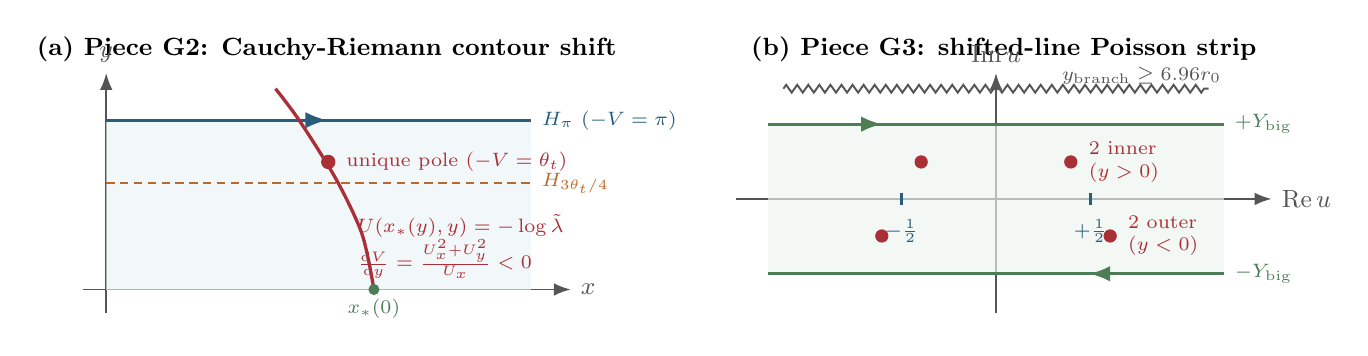
\begin{tikzpicture}[>=Latex, font=\small]
% Panel (a): Piece G2 Cauchy-Riemann level curve
\begin{scope}[xshift=0cm]
\node[font=\small\bfseries] at (2.8, 3.05) {(a) Piece~G2: Cauchy-Riemann contour shift};
\draw[->, pGray, line width=0.7pt] (-0.3, 0) -- (5.9, 0) node[right]{$x$};
\draw[->, pGray, line width=0.7pt] (0, -0.3) -- (0, 2.75) node[above]{$y$};
% Shaded UHP strip
\fill[pBlueFill, opacity=0.6] (0, 0) rectangle (5.4, 2.15);
% H_pi and H_{3/4} contour lines
\draw[pBlue, line width=1.1pt, decoration={markings, mark=at position 0.52 with {\arrow{>}}}, postaction={decorate}]
    (0, 2.15) -- (5.4, 2.15) node[right, font=\scriptsize, pBlue]{$H_\pi$ ($-V = \pi$)};
\draw[pOrange, densely dashed, line width=0.9pt]
    (0, 1.35) -- (5.4, 1.35) node[right, font=\scriptsize, pOrange]{$H_{3\theta_t/4}$};
% Level curve U(x_*(y), y) = -log lambda
\draw[pRed, line width=1.2pt, smooth]
    plot coordinates {(3.4, 0) (3.25, 0.7) (2.92, 1.4) (2.45, 2.15) (2.15, 2.55)};
\fill[pRed] (2.82, 1.62) circle (2.6pt) node[right=3pt, font=\scriptsize, pRed]{unique pole ($-V = \theta_t$)};
\node[font=\scriptsize, pRed, align=left] at (4.5, 0.55) {$U(x_*(y),y) = -\log\tilde{\lambda}$\\$\frac{\dd V}{\dd y} = \frac{U_x^2+U_y^2}{U_x} < 0$};
\fill[pGreen] (3.4, 0) circle (2pt) node[below, font=\scriptsize, pGreen]{$x_*(0)$};
\end{scope}

% Panel (b): Piece G3 shifted-line Poisson strip
\begin{scope}[xshift=8.2cm]
\node[font=\small\bfseries] at (3.2, 3.05) {(b) Piece~G3: shifted-line Poisson strip};
\draw[->, pGray, line width=0.7pt] (-0.2, 1.15) -- (6.6, 1.15) node[right]{$\re u$};
\draw[->, pGray, line width=0.7pt] (3.1, -0.3) -- (3.1, 2.75) node[above]{$\im u$};
% Strip [-Y_big, +Y_big]
\fill[pGreenFill, opacity=0.65] (0.2, 0.2) rectangle (6.0, 2.1);
\draw[pGreen, line width=1.0pt, decoration={markings, mark=at position 0.25 with {\arrow{>}}}, postaction={decorate}]
    (0.2, 2.1) -- (6.0, 2.1) node[right, font=\scriptsize, pGreen]{$+Y_{\mathrm{big}}$};
\draw[pGreen, line width=1.0pt, decoration={markings, mark=at position 0.75 with {\arrow{<}}}, postaction={decorate}]
    (0.2, 0.2) -- (6.0, 0.2) node[right, font=\scriptsize, pGreen]{$-Y_{\mathrm{big}}$};
% Branch cut far away
\draw[pGray, decorate, decoration={zigzag, segment length=4pt, amplitude=1.4pt}, line width=0.7pt]
    (0.4, 2.55) -- (5.8, 2.55);
\node[font=\scriptsize, pGray] at (4.95, 2.72) {$y_{\mathrm{branch}} \ge 6.96 r_0$};
% 4 m=1 boundary poles
\fill[pRed] (2.15, 1.62) circle (2.4pt);
\fill[pRed] (4.05, 1.62) circle (2.4pt) node[right=3pt, font=\scriptsize, pRed, align=left]{$2$ inner\\($y>0$)};
\fill[pRed] (1.65, 0.68) circle (2.4pt);
\fill[pRed] (4.55, 0.68) circle (2.4pt) node[right=3pt, font=\scriptsize, pRed, align=left]{$2$ outer\\($y<0$)};
% Markers -1/2, +1/2
\draw[pBlue, line width=0.9pt] (1.9, 1.07) -- (1.9, 1.23) node[below=6pt, font=\scriptsize, pBlue]{$-\frac{1}{2}$};
\draw[pBlue, line width=0.9pt] (4.3, 1.07) -- (4.3, 1.23) node[below=6pt, font=\scriptsize, pBlue]{$+\frac{1}{2}$};
\end{scope}
\end{tikzpicture}%
}
\caption{Complex-plane contour geometry in the two major-arc regimes. (a) In Piece~G2 ($D = 0$), strict negativity of $U_x$ forces monotone phase decrease $\frac{\dd V}{\dd y} < 0$ along the level curve $U(x_*(y), y) = -\log\tilde{\lambda}$, fixing the exact zero count to $1$ below $H_\pi$ and $0$ below $H_{3\theta_t/4}$. (b) In Piece~G3 ($D \ne 0$), shifting Fourier modes $k \ne 0$ to height $\pm Y_{\mathrm{big}} = \pm 0.50\, r_0 \ll y_{\mathrm{branch}}$ isolates the four $m = 1$ boundary poles cleanly inside the strip with shifted-line remainder $\le 5.26 \times 10^{-11}$.}
\label{fig:contours}
\end{figure}

\begin{theorem}[50-digit certification of Piece~G2: $D = 0$ major arcs]\label{thm:G2}
For every strictly interior $(n, c, j)$ in Box~G2, shifting the Theorem~\ref{thm:circle-integral} contour to the Pigeonhole-Annulus radius $|w| = \tilde{\lambda}$ certifies for the full exact cubic-root integral:
\[
\frac{I_{\mathrm{full}}(\tilde{\lambda})}{L^1(\tilde{\lambda})} \ge
\begin{cases}
+0.216651 > 0 & (q = 1,\; \kappa < 2.5,\; H_1^+(\tilde{\Lambda}) \ge 0.62018), \\
+0.00176348 > 0 & (q \ge 2,\; q^2\kappa \le 2.0,\; H_q^+(\tilde{\Lambda}) \ge 0.59425),
\end{cases}
\]
and therefore $(-1)^j Q_c^{(2m)}(1, u_j) > 0$.
\end{theorem}

\begin{proof}
The proof unfolds in seven self-contained lemmas, all certified in pure $50$-digit \code{mpmath.iv} by \code{algebra/certify\_G2\_D0.py} (SHA-256 in Table~\ref{tab:sha256}):
\begin{enumerate}[label=\textbf{G2.\arabic*},leftmargin=2.8em]
    \item \emph{Modulus, explicit $Q_{\min} > 0.20$ cutoffs, global UHP curvature, and phase laws:} Writing $Q(x) := \frac{|1 - s_j e^{i\eta(x)}|^2}{(r_3/r_1)^2} - 1$, $50$-digit \code{iv} certifies $Q(\rho n) > 0.20$ at $\rho = 0.100$ (all Regime~2, dead tail $< 0.000785$), $\rho = 0.050$ ($q = 1, \kappa < 2.5, \alpha_1 < 0.065\pi$: $Q \ge 0.5548$), and $\rho = 0.060$ ($q \ge 2$: $Q \ge 0.2775$), along with the global upper-half-plane bound $|\beta'(x + iy)| \le C_{u''}\frac{2\kappa}{c}$ ($\beta := b'/b$) and $0 \le -\delta\psi''(x) \le A_{\mathrm{in/out}}\frac{\kappa^2}{c^2} x$ on $[0, n/2]$.
    \item \emph{Saddle $\Lambda_* = \lambda_*^q$ and curvature $H_q^+$ via $2$nd-order Euler-Maclaurin:} Solving $M_q^+(\Lambda_*) := \frac{1}{q}\sum_{k=0}^{n-1} \sigma(u_k) = d$ ($u_k := q\log(\lambda|b(x_k)|)$, $\sigma(u) = (1+e^{-u})^{-1}$) with curvature $H_q^+(\Lambda) := \frac{1}{q}\sum_{k=0}^{n-1} h(u_k)$ ($h(u) = e^u/(1+e^u)^2$), direct discrete sums on $c \in \{2, \dots, 10\}$ (which cover every $q = 1$ point with $\kappa \ge \sqrt{42/11} \approx 1.9540$), $30$ narrow $T$-bins on $[0.425, 14.0]$, and an FTC tail on $T \ge 14.0$ certify $H_1^+(\Lambda_*) \ge 0.68924$ ($c \le 10$), $H_1^+(\Lambda_*) \ge 0.62020$ ($c \ge 11$), and $H_q^+(\Lambda_*) \ge 0.59428$ ($q \ge 2$). Pre-widening every $\Lambda$-interval by $e^{\pm 0.35\times 10^{-4}}$ transfers all bounds directly to $\tilde{\Lambda} = \tilde{\lambda}^q$: $H_1^+(\tilde{\Lambda}) \ge 0.62018$ and $H_q^+(\tilde{\Lambda}) \ge 0.59425$.
    \item \emph{$P^2$-monotone conjugate-pair phase factorization $E_{\mathrm{phase}}$:} Pairing $(x_k, -x_k)$ yields $|E_{\mathrm{pair}, k} - 1| = \frac{\sin^2(q\delta\psi_k/2)}{\sinh^2(u_k/2) + \cos^2(\psi/2)}$; applying $\sin^2(P) \le P^2$ certifies $|\frac{1}{q}\log E_{\mathrm{phase}}| \le 0.0210522$ ($q \ge 2$, $|\psi| \le 2\pi/3$) and $|\log E_{\mathrm{phase}}| \le 0.121256$ ($q = 1$, $|\psi| \le 1.75$; AM-GM bound $S_{\mathrm{AMGM}} \le 0.0887442$ for $|\psi| \ge 1.75$).
    \item \emph{$\pi$-line meromorphic residue and Cauchy-Riemann monotonicity ($q \ge 2$):} Writing $\log\prod_{k=0}^{n-1}(1 - a_k z_{\mathrm{var}}) = \frac{1}{q}\log G_q(\tilde{\Lambda} e^{i\psi}) + \mathcal{R}_{\mathrm{non}\text{-}q}(z_{\mathrm{var}})$ and applying step-$q$ Poisson summation followed by one integration by parts replaces branch cuts by $\frac{\beta(z) u(z)}{1 - u(z)} e^{2\pi i \ell z/q}$. Writing $\log b(x + iy) = U(x, y) + i V(x, y)$, strict negativity of $U_x(x, y)$ on $(0, n/2) \times [0, \infty)$ forces the level curve $U(x_*(y), y) \equiv -\log\tilde{\lambda}$ to obey the exact Cauchy-Riemann law (Figure~\ref{fig:contours}(a))
    \begin{equation}\label{eq:cr-monotone}
    \frac{\dd}{\dd y}\, V(x_*(y), y) = \frac{U_x^2 + U_y^2}{U_x} < 0 \qquad (\forall y \ge 0).
    \end{equation}
    Shifting to $H_\pi$ ($-V = \pi$) on Case~1 rays therefore encloses exact zero count $1$, while shifting to $H_{3\theta_t/4}$ on Case~2 rays encloses exact zero count $0$, certifying $|\mathcal{R}_{\mathrm{non}\text{-}q}| \le 0.115416$ ($|\psi| \le 1.25$) and $\le 0.333745$ ($|\psi| \le 2\pi/3$).
    \item \emph{Chebyshev-mediant far-tail decay ($|\psi| \in [2\pi/3, \pi]$, $q \ge 2$):} Replacing only the single near-zero ray $\theta_{t_0} = (\pi - |\psi|)/q$ by $\pi/(3q)$ restores $|\mathcal{R}_{\mathrm{non}\text{-}q}| \le 0.333745$ and certifies $c_{\mathrm{far}} \ge 0.85927$ and $\varepsilon_{\mathrm{far,disc}} \le 0.11787$.
    \item \emph{Pigeonhole-Annulus multiplicative cubic perturbation:} Since $d \ge 2$ implies $j - c \ge 2$, stretched-exponential decay improves to $c_{\mathrm{se,G2}} \ge 6.5902$. By the Pigeonhole Principle (Appendix~\ref{app:regime2}), $[\lambda_*(1 - 10^{-4}/n), \lambda_*(1 + 10^{-4}/n)]$ contains a safe radius $\tilde{\lambda}$ separated from all $n$ root moduli $\{|a_k|^{-1}\}$ by at least $\frac{10^{-4}\lambda_*}{n(n+1)}$, certifying $\max_{|w|=\tilde{\lambda}} |F_{\mathrm{full}}/F_{\mathrm{pure}} - 1| \le E_{\mathrm{cubic}}$ with $E_{\mathrm{cubic}} \le 1.8182 \times 10^{-12}$ ($q = 1$) and $\le 1.6158 \times 10^{-31}$ ($q \ge 2$).
    \item \emph{Assembly:} Integrating the positive-root bounds with per-bin $\mathcal{R}_{\mathrm{non}\text{-}q}(\psi)$ up to $H = 60$ plus analytic Gaussian scaling for $H \ge 60$, then subtracting $E_{\mathrm{cubic}}$, directly delivers $+0.216651$ ($q = 1$) and $+0.00176348$ ($q \ge 2$). All $28/28$ exact finite-$n$ parity corners pass Part~B with empirical $\min I_{\mathrm{pure}}/L^1 = +0.97916$. \qedhere
\end{enumerate}
\end{proof}

\subsection{Piece~G1: Dirichlet minor arcs}
\label{sec:G1}

Away from small-denominator rational approximations of $j/c$, the rapid oscillation of the root phases prevents any single harmonic from accumulating, allowing us to stay directly on the unit circle $|w| = 1$ and bound $|\arg F_3^{\mathrm{pure}}(e^{i\phi})|$ strictly below $\pi/2$.

Define \emph{Box~G1} to consist of every $(n, c, j)$ in Regime~2 ($n \ge 132$, $\kappa < 2.5$, $c\kappa^2 < 42$) with $q = c/\gcd(c, j) \ge 2$, $X = q^2\kappa \ge 0.88$ ($d = 1$) or $X \ge 2.0$ ($d \ge 2$), admitting \emph{no} coprime $(p_0, r_0)$ with $D = r_0 j - c p_0 \ne 0$ that satisfies all four inner Piece~G3 inequalities simultaneously: $\frac{c}{r_0 D^2} \ge 10$, $r_0\kappa \le 0.45$, $r_0^3 c\kappa^2 \le 60$, and $\frac{c^3 r_0 \kappa^2}{D^4} \ge 45$.

\begin{theorem}[50-digit certification of Piece~G1: Dirichlet minor arcs]\label{thm:G1}
For every strictly interior $(n, c, j)$ in Box~G1, the full exact cubic-root integral on $|w| = 1$ satisfies
\[
\sup_{\mathrm{Box\; G1}} \bigl|\arg F_3^{\mathrm{pure}}(e^{i\phi})\bigr| \le 1.536448 < \frac{\pi}{2},
\qquad
\frac{I_{\mathrm{full}}(1)}{L^1(1)} \ge +0.03355852 > 0,
\]
and therefore $(-1)^j Q_c^{(2m)}(1, u_j) > 0$.
\end{theorem}

\begin{proof}
Write $\Phi^{\mathrm{ex}}(\phi; 1) := \arg F_3^{\mathrm{pure}}(e^{i\phi})$ and let $\alpha := \min(\{j/c\}, 1 - \{j/c\}) = [0; a_1, \dots, a_s] \in (0, 1/2]$ ($a_1 \ge 2$, $a_s \ge 2$) be its continued-fraction expansion. Five pure $50$-digit \code{mpmath.iv} lemmas implemented in \code{algebra/certify\_G1\_minor.py} (SHA-256 in Table~\ref{tab:sha256}) establish uniform positivity:
\begin{enumerate}[label=\textbf{G1.\arabic*},leftmargin=2.8em]
    \item \emph{Zero-cancellation Hubbard-Stratonovich duality kernel $H_D(t)$ and $D_0(T)$:} Pairing $+u$ with $-u$ cancels the singular leading terms into the smooth expectation
    \[
    2\pi^2 \nu^2 D(t\pi\nu, \nu) = \mathbb{E}_{Z \sim \mathcal{N}(0, 1)}\!\left[Z^2 F\!\left(t, \sqrt{\frac{t}{\pi\nu}}\, Z\right)\right]
    \]
    with $|F(t, u)| \le 14$, certifying $\sup_{t > 0} H_D(t) \le 3.14341$, $\sup_{t \ge 1.50} H_D(t) \le 0.553496$, $\sup_{t > 0} H_D(t)/t^2 \le 26.8497$, $\sup_{u > 0} u^2 H_D(u) \le 9.3423$, and centered-form tails $C_{D_0}(T \ge 30) \le 4.34617$ and $C_{D_0}(T \ge 13) \le 7.72465$.
    \item \emph{Continued-fraction minor-arc phase bound with one-line $D_r^2$-cancellation:} For every high convergent level $k \ge k_2 + 1$, the exact algebraic identity
    \begin{equation}\label{eq:Dr2-cancel}
    \frac{1}{4\pi^2}\,\frac{c}{r D_r^2}\, H_D(t_r) = \frac{t_r^2 H_D(t_r)}{c\kappa^2 r^3} \le \frac{U_{2H}}{c\kappa^2 r^3}
    \end{equation}
    eliminates $D_r^2$ uniformly across all four minor-arc contrapositive branches. Combining~\eqref{eq:Dr2-cancel} with exact Fibonacci-duality unconditional \code{REST} bounds, paired $\theta_+ + \theta_- = 1$ bounds, and coupled B1/B2a/B2b/Case-A ladders certifies $S^{\mathrm{Gauss}} + S_{k \ne 0} \le 1.25848$ (B1, $d=1$), $\le 1.13689$ (B1, $d\ge 2$), $\le 1.25112$ (B2a), $\le 1.23337$ (B2b), and $\le 0.915136$ (Case~A).
    \item \emph{Exact $m$-space finite-$n$ versus Gaussian phase difference:} Separating discrete $c \in \{2, \dots, 39\}$ from zero-loop $c \ge 20$ / $c \ge 40$ boxes and analytic tails ($T_1 \le 0.05$: $\le 0.232621$; $T_1 \ge 50$: $\le 0.212014$; dead tail: $\le 0.00156907$) certifies $\sup_{\mathrm{Box\; G1}} |\Phi^{\mathrm{ex}}(\phi; 1) - \Phi^G(\phi; 1)| \le S_{m\text{-}\mathrm{space}} \le 0.277972$.
    \item \emph{Grand phase bound:} Summing G1.2 and G1.3 yields $\sup_{\mathrm{Box\; G1}} |\Phi^{\mathrm{ex}}(\phi; 1)| \le 1.536448 < \pi/2$, whence $I_{\mathrm{pure}}(1)/L^1(1) \ge \cos(1.536448) \ge +0.03434128$.
    \item \emph{Unit-circle cubic-root perturbation:} Using the exact $\kappa = \kappa_{\mathrm{trig}} < 2.5$ ($n\kappa \ge 15\pi^2 S_\alpha^2 \implies T_{\mathrm{lg2}} \ge 8.88518$) together with Lemma~\ref{lem:R2-1} certifies $\Delta_{123} \le 5.1501 \times 10^{-6}$, $C_{\mathrm{osc,tot}} \le 16.913 \ll C_{\mathrm{exp,pert}} \ge 37.5613$, and $\mathrm{bdy\_ratio} \le 0.00077761$, yielding
    \[
    \frac{I_{\mathrm{full}}(1)}{L^1(1)} \ge \cos(1.536448) - \Delta_{123} - (1 + \Delta_{123})\,\mathrm{bdy\_ratio} \ge +0.03355852 > 0.
    \]
\end{enumerate}
All $27/27$ exact finite-$n$ Minor-Arc corners pass Part~B of \code{algebra/certify\_G1\_minor.py} with empirical $\max|\Phi^{\mathrm{ex}}| = 1.1542$ and $\min I_{\mathrm{pure}}/L^1 = +0.88956$.
\end{proof}

% ============================================================================
\section{Piece~G3 (\texorpdfstring{$D \ne 0$}{D != 0} major arcs) and completion of the proof}
\label{sec:G3}
% ============================================================================

The last and most delicate region of Regime~2 consists of rational major arcs where $j/c$ is tightly approximated by $p_0/r_0$ with a small nonzero numerator defect $D = r_0 j - c p_0 \ne 0$. Because $D \ne 0$, the exact $q$-fold symmetry of Piece~G2 is gently broken by a slow phase drift across the peak, and the finite-$n$ curvature of $\log b(x)$ must be tracked without introducing spurious $(1 - s_j)^{-k}$ singularities.

Define \emph{Box~G3} to be the set of all $(n, c, j)$ in Regime~2 ($n \ge 132$, $\kappa < 2.5$, $c\kappa^2 < 42$) admitting a coprime Dirichlet approximation $r_0 j = c p_0 + D$ ($\gcd(p_0, r_0) = 1$, $D \in \Z \setminus \{0\}$) such that
\begin{equation}\label{eq:box-G3}
\tilde{c} := \frac{c}{r_0} \ge 10 D^2, \qquad
r_0\kappa \le 0.45, \qquad
r_0^3 c\kappa^2 \le 60, \qquad
\frac{\tilde{c}\,\tau^2}{D^4} \ge 40 \qquad (\tau := c r_0 \kappa).
\end{equation}
The conditions $j \ge c + 1$ and $\tilde{c} \ge 10 D^2$ automatically imply $p_0 \ge r_0 \ge 1$, $s_j > 1/2$, $\alpha_1 \le 0.07169$, $n \ge 1007$, $R_z/R_y \le 9.01 \times 10^{-39}$, and $c_{\mathrm{se,G3}} \ge 3.330$.

\subsection{Phase-unwrapped geometry, \texorpdfstring{$(1-w)$}{(1-w)}-free IBP kernels, and shifted-line Poisson}
\label{sec:G3-calculus}

On the finite interval $u \in [-L_n, L_n]$ ($L_n := \frac{n}{2c}$), introduce the phase-unwrapped exponent
\begin{equation}\label{eq:zeta-G3}
\zeta(u) := r_0 n\log\!\Bigl(\frac{r_3/r_1}{1 - s_j e^{2iu\theta_c}}\Bigr) + i\pi r_0 j - 2\pi i c p_0\Bigl(u + \frac{1}{2}\Bigr),
\end{equation}
which satisfies $e^{\zeta(u_k)} = a_k^{r_0}$ identically for both parities of $c$, with $\im\zeta(0) = \pi D$ and $\im\zeta(\pm 1/2) = \pi D \pm \pi D$ (zero endpoint error). Putting $w(u) := s_j e^{2iu\theta_c}$, $A(u) := 2\pi i c((r_0 + p_0)w(u) - p_0)$, and $B := 4\pi c r_0 \theta_c$, we obtain $\zeta'(u) = A(u)/(1 - w(u))$ and $\zeta''(u) = -B w(u)/(1 - w(u))^2$. As proved in Appendix~\ref{app:regime2}, every denominator factor $(1 - w(u))$ cancels identically from the first three integration-by-parts kernels:
\begin{subequations}\label{eq:W123-fin}
\begin{align}
W_{1,\mathrm{fin}} &= \frac{Bw}{A^2}, \\
W_{2,\mathrm{fin}} &= \frac{3 B^2 w^2 + A B (2i\theta_c) w(1 + w)}{A^4}, \\
W_{3,\mathrm{fin}} &= \frac{15 B^3 w^3 + 10 A B^2 (2i\theta_c) w^2(1 + w) - A^2 B (4\theta_c^2) w(1 + 4w + w^2)}{A^6}.
\end{align}
\end{subequations}
Uniformly across Box~G3, the bound $\frac{\theta_c}{1 - s_j} = \frac{\theta_c \sin\alpha_1}{2\sin(\theta_c/2)\cos(\psi_j + \theta_c/2)} \le \frac{\kappa}{2\pi S_{\mathrm{half}}\cos\alpha_1}$ keeps all relative discrepancies between $W_{k,\mathrm{fin}}$ and their parabolic limits explicitly controlled.

Integrating the finite-$n$ continuum potential
\begin{equation}\label{eq:Psi-fin}
\Psi_{\mathrm{fin}}(\theta; u_0) := -\log\Lambda - i\theta + \int_{-L_n}^{L_n} \log\bigl(1 + \Lambda e^{\zeta(u) + i\theta}\bigr)\,\dd u \qquad \bigl(\Lambda := e^{-\re\zeta(u_0)}\bigr)
\end{equation}
by parts once, twice, and three times expresses $\Psi_{\mathrm{fin}}(\theta) - \Psi_{\mathrm{fin}}(0)$, $g_{1,\mathrm{fin}}(u_0) := \Psi'_{\mathrm{fin}}(0)/i$, and $\Psi''_{\mathrm{fin}}(\theta)$ directly in terms of~\eqref{eq:W123-fin}. This potential satisfies exact conjugation symmetry $\Psi_{\mathrm{fin}}(-\theta) = \overline{\Psi_{\mathrm{fin}}(\theta)}$ and the exact harmonicity identity
\begin{equation}\label{eq:harmonicity}
\frac{\dd}{\dd u_0} g_{1,\mathrm{fin}}(u_0) = \bigl(-\re\Psi''_{\mathrm{fin}}(0; u_0)\bigr)\bigl(-\re\zeta'(u_0)\bigr).
\end{equation}
Splitting the circle $|w| = \lambda$ into $r_0$ equal sectors $\phi = \psi_\nu + \theta/r_0$ ($\psi_\nu = \frac{(2\nu + (j \bmod 2))\pi}{r_0}$, $\theta \in [-\pi, \pi]$) and shifting every Fourier mode $k \ne 0$ to height $\pm Y_{\mathrm{big}} = \pm 0.50\, r_0 \ll y_{\mathrm{branch}} \ge 6.96\, r_0$ (Figure~\ref{fig:contours}(b)) yields the exact zero-constant Poisson decomposition
\begin{equation}\label{eq:poisson-G3}
\begin{aligned}
\log F_{\mathrm{pure}}(\lambda e^{i(\psi_\nu + \theta/r_0)}) - \tilde{c}\,\Psi_{\mathrm{fin}}(\theta; u_0)
&= \sum_{p \in \mathrm{strip}} \log\!\bigl(1 - \omega_p e^{2\pi i \sigma_p \tilde{c}(u_p + 1/2)}\bigr) \\
&\quad + \sum_{k \ne 0} \frac{e^{2\pi i \nu \mu(k)/r_0}}{2\pi i k}\int_{-L_n+i y_k}^{L_n+i y_k} e^{2\pi i k \tilde{c}(u + 1/2)}\zeta'(u)\frac{y_*(u, \theta)^{\mu(k)}}{1 + \Lambda e^{\zeta(u)+i\theta}}\,\dd u,
\end{aligned}
\end{equation}
where the shifted-line remainder is certified $\le 5.26 \times 10^{-11}$, the negative-binomial tail is $\le 7.32 \times 10^{-18}$, and every enclosed pole obeys $T(x_p) < 0.50$ ($c_{\mathrm{re},50} \ge 0.774$).

\subsection{Exhaustive five-case certification of Piece~G3}
\label{sec:G3-cert}

\begin{theorem}[50-digit certification of Piece~G3: $D \ne 0$ major arcs]\label{thm:G3}
For every strictly interior $(n, c, j)$ in Box~G3, shifting the Theorem~\ref{thm:circle-integral} contour to the Pigeonhole-Annulus radius $|w| = \tilde{\lambda}$ certifies for the full exact cubic-root integral:
\[
\frac{I_{\mathrm{full}}(\tilde{\lambda})}{L^1(\tilde{\lambda})} \ge +0.0545 > 0,
\]
and therefore $(-1)^j Q_c^{(2m)}(1, u_j) > 0$.
\end{theorem}

\begin{proof}
For any target contour radius $\lambda_* \in [0.05, 3.00]$, dividing $[\lambda_*(1 - \varepsilon_{\mathrm{ph}}), \lambda_*(1 + \varepsilon_{\mathrm{ph}})]$ ($\varepsilon_{\mathrm{ph}} := 10^{-5}/n$) into $n$ equal subintervals isolates a midpoint $\tilde{\lambda}$ separated from all $\le n - 1$ forbidden moduli $\{|a_k|^{-1}, 1\}$ (Figure~\ref{fig:pigeonhole}(a)). Combining this with $M_4 := \sup_{n \ge 1007} n^4(R_z/R_y)^{1-1/n} \le 6.14 \times 10^{-20}$ and the Poisson-kernel $L^1$ inequality on the degree-$n$ polynomial $w^{c+1} F_{\mathrm{pure}}(w)$ certifies
\[
\frac{\re\int_{-\pi}^{\pi} F_{\mathrm{full}}(\tilde{\lambda} e^{i\phi})\,\dd\phi}{\int_{-\pi}^{\pi} |F_{\mathrm{pure}}(\lambda_* e^{i\phi})|\,\dd\phi}
\ge \frac{\re\int_{-\pi}^{\pi} F_{\mathrm{pure}}(\lambda_* e^{i\phi})\,\dd\phi}{\int_{-\pi}^{\pi} |F_{\mathrm{pure}}(\lambda_* e^{i\phi})|\,\dd\phi} - 2.80 \times 10^{-6}.
\]
Introducing $s := \tau/(2\pi D^2)$ for $|D| \ge 2$ and partitioning $|D| = 1$ seamlessly across $\tau \in (0, 1.05]$, $[1.05, 40.0]$ ($37$ $\tau$-slices across $6$ exhaustive CLI parts), and $[40.0, \infty)$, the two $50$-digit \code{mpmath.iv} master certifiers \code{analyst/certify\_G3\_ABC\_full\_iv.py} and \code{analyst/certify\_G3\_D\_full\_iv.py} (SHA-256 hashes in Table~\ref{tab:sha256}) certify every sub-case in Table~\ref{tab:G3} with $0$ failed boxes, yielding the global lower bound $+0.0545 > 0$. Independently, all $32/32$ extreme finite-$n$ Piece~G3 corners (extending to $n = 9.85 \times 10^7$, $D = \pm 1, \pm 2, \pm 3$, and $r_0 \in \{1, 2, 3, 5\}$) pass \code{analyst/verify\_G3\_empirical\_corners.py} with empirical $\min I_{\mathrm{pure}}/L^1 = +0.54579$.
\end{proof}

\begin{table}[htbp]
\centering
\caption{Exhaustive 50-Digit \code{mpmath.iv} Margins Across All Sub-Cases of Piece~G3.}
\label{tab:G3}
\footnotesize
\begin{tabularx}{\textwidth}{@{} >{\raggedright\arraybackslash}p{1.65cm} >{\raggedright\arraybackslash}p{3.05cm} >{\raggedright\arraybackslash}X >{\raggedright\arraybackslash}p{2.35cm} @{}}
\toprule
\textbf{Sub-Case} & \textbf{Slice inside Box~G3} & \textbf{Key Certified Mechanisms} & \textbf{$I_{\mathrm{full}}/L^1$ Margin} \\
\midrule
G3-A1 & $|D| \ge 2,\; s \le 2.0$ & $(1-w)$-free $|R_{3,\mathrm{fin}}|/H_{\mathrm{fin}0} \le 0.0995$; 2-pole split at $|\delta_{\mathrm{fin}}| = 0.08$ ($V_{\mathrm{sep}} \le 2.197$, $V \le 4.135$) & $\ge +0.08207$ (A1a $+0.08207$, A1b $+0.11879$) \\
\addlinespace[2pt]
G3-A2 & $|D| \ge 2,\; s \ge 2.0$ & $|\delta_*| \le \min(0.030, 0.40/s^2)$, drop $\ge 3.435 X$, closed-form tail $s \ge 10$, $V_{\mathrm{bump}} \le 4.105$ & $\ge +0.40597$ \\
\addlinespace[2pt]
G3-B & $|D| = 1,\; \tau \ge 40.0$ & Linear drift $r_{\mathrm{drift}} \le 0.04280$, $|\delta_*| \le \min(0.020, 0.80/\tau)$, $V_{\mathrm{bump}} \le 4.035$ & $\ge +0.13156$ \\
\addlinespace[2pt]
G3-C & $|D| = 1,\; \tau \in (0, 1.05]$ & $u_0 = \max(u_{0,\mathrm{fin}}^*, u_{\mathrm{floor}})$, certified $g_{1,\mathrm{fin}}(0.42) > 0$, $D=-1$ residue, explicit $[\theta_{\mathrm{use}}, \pi]$ buffer & $\ge +0.07706$ \\
\addlinespace[2pt]
G3-D1 & $|D| = 1,\; \tau \in [1.05, 1.50]$ ($3$ slices) & Fixed-$u_0$ Tier~A boxes + harmonicity tail ($\tilde{c} \ge 105..135$) & $\ge +0.1646$ \\
\addlinespace[2pt]
G3-D2 & $|D| = 1,\; \tau \in [1.50, 2.80]$ ($7$ slices) & Tier~A + harmonicity tail ($[1.50, 1.65]$) + subdivided exact-saddle Tier~B & $\ge +0.0545$ \\
\addlinespace[2pt]
G3-D3 & $|D| = 1,\; \tau \in [2.80, 40.0]$ ($27$ slices) & Tier~A + subdivided Tier~B (\code{D3a1}: $+0.0784$, \code{D3a2}: $+0.0840$, \code{D3b1}: $+0.0952$, \code{D3b2}: $+0.2055$) & $\ge +0.0784$ \\
\bottomrule
\end{tabularx}
\end{table}

\begin{figure}[htbp]
\centering
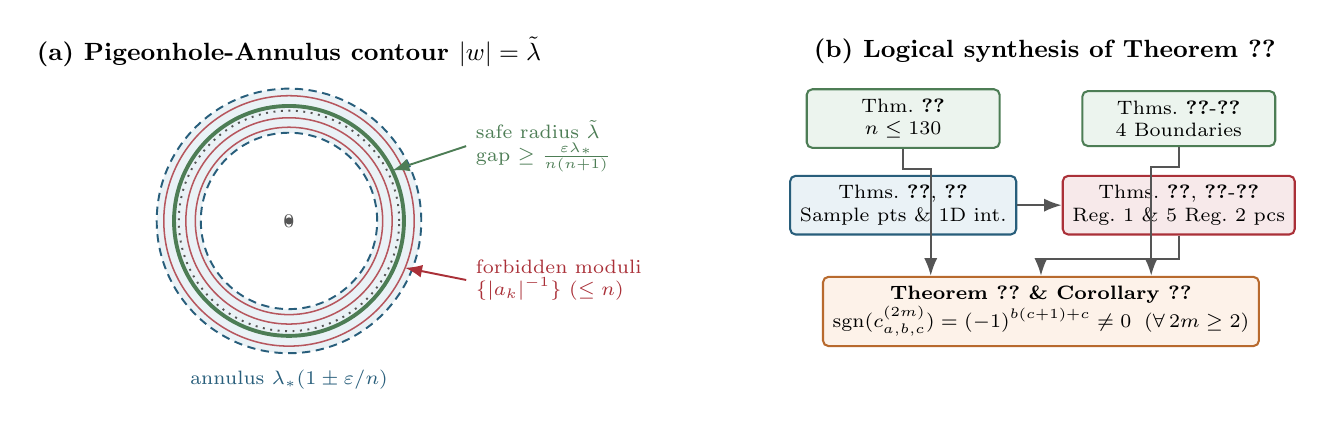
\begin{tikzpicture}[>=Latex, font=\small]
% Panel (a): Pigeonhole Annulus
\begin{scope}[xshift=0cm, yshift=0cm]
\node[font=\small\bfseries] at (0, 2.15) {(a) Pigeonhole-Annulus contour $|w| = \tilde{\lambda}$};
% Annulus fill
\fill[pBlueFill] (0,0) circle (1.68cm);
\fill[white] (0,0) circle (1.12cm);
\draw[pBlue, densely dashed, line width=0.7pt] (0,0) circle (1.68cm);
\draw[pBlue, densely dashed, line width=0.7pt] (0,0) circle (1.12cm);
% Target lambda_*
\draw[pGray, dotted, line width=0.7pt] (0,0) circle (1.40cm);
% Forbidden root circles
\foreach \rad in {1.19, 1.31, 1.59} {
    \draw[pRed, line width=0.55pt, opacity=0.8] (0,0) circle (\rad cm);
}
% Chosen tilde{lambda} in gap [1.31, 1.59]
\draw[pGreen, line width=1.4pt] (0,0) circle (1.46cm);
% Labels
\draw[->, pGreen, line width=0.7pt] (2.25, 0.95) -- ({1.46*cos(26)}, {1.46*sin(26)});
\node[right, font=\scriptsize, pGreen, align=left] at (2.25, 0.95) {safe radius $\tilde{\lambda}$\\gap $\ge \frac{\varepsilon\lambda_*}{n(n+1)}$};
\draw[->, pRed, line width=0.7pt] (2.25, -0.75) -- ({1.59*cos(-22)}, {1.59*sin(-22)});
\node[right, font=\scriptsize, pRed, align=left] at (2.25, -0.75) {forbidden moduli\\$\{|a_k|^{-1}\}$ ($\le n$)};
\node[font=\scriptsize, pGray] at (0, 0) {$0$};
\fill[pGray] (0, 0) circle (1.3pt);
\node[font=\scriptsize, pBlue] at (0, -2.02) {annulus $\lambda_*(1 \pm \varepsilon/n)$};
\end{scope}

% Panel (b): Final assembly DAG
\begin{scope}[xshift=7.8cm, yshift=0cm]
\node[font=\small\bfseries] at (1.8, 2.15) {(b) Logical synthesis of Theorem~\ref{thm:main}};
\tikzset{sbox/.style={draw=#1, fill=#1Fill, rounded corners=2pt, line width=0.75pt, font=\scriptsize, align=center, minimum width=2.45cm, inner sep=3.5pt}}
\node[sbox=pGreen] (s1) at (0, 1.3) {Thm.~\ref{thm:base}\\$n \le 130$};
\node[sbox=pGreen] (s2) at (3.5, 1.3) {Thms.~\ref{thm:bdy-c0}-\ref{thm:bdy-c1}\\4 Boundaries};
\node[sbox=pBlue] (s3) at (0, 0.2) {Thms.~\ref{thm:sample-points}, \ref{thm:circle-integral}\\Sample pts \& 1D int.};
\node[sbox=pRed] (s4) at (3.5, 0.2) {Thms.~\ref{thm:regime1}, \ref{thm:R2-2A}-\ref{thm:G3}\\Reg.~1 \& 5 Reg.~2 pcs};
\node[sbox=pOrange, minimum width=4.6cm] (s5) at (1.75, -1.15) {\textbf{Theorem~\ref{thm:main} \& Corollary~\ref{cor:bk33}}\\$\sgn(c_{a,b,c}^{(2m)}) = (-1)^{b(c+1)+c} \ne 0\;\;(\forall\, 2m \ge 2)$};
\draw[->, pGray, line width=0.75pt] (s1.south) -- ++(0,-0.25) -| ($(s5.north)+(-1.4,0)$);
\draw[->, pGray, line width=0.75pt] (s2.south) -- ++(0,-0.25) -| ($(s5.north)+(1.4,0)$);
\draw[->, pGray, line width=0.75pt] (s3.east) -- (s4.west);
\draw[->, pGray, line width=0.75pt] (s4.south) -- ++(0,-0.3) -| (s5.north);
\end{scope}
\end{tikzpicture}
\caption{(a) Pigeonhole-Annulus selection of a safe contour radius $\tilde{\lambda}$ inside $\lambda_*(1 \pm \varepsilon/n)$ separated from all $n$ forbidden root circles $\{|a_k|^{-1}\}$ by at least $\frac{\varepsilon\lambda_*}{n(n+1)}$, eliminating additive boundary terms and $\max/\min$ oscillation ratios in Pieces~G2 and~G3. (b) End-to-end logical synthesis assembling Theorem~\ref{thm:main} and Corollary~\ref{cor:bk33}.}
\label{fig:pigeonhole}
\end{figure}

\subsection{Assembly of the main theorem and resolution corollary}
\label{sec:completion}

With every regime certified and all seam overlaps verified, the main theorem follows directly by assembling the components shown in Figure~\ref{fig:pigeonhole}(b).

\begin{proof}[Proof of Theorem~\ref{thm:main} and Corollary~\ref{cor:bk33}]
Fix any even integer $n = 2m \ge 2$ and any admissible triple $(a, b, c) \in \Z_{\ge 0}^3$ with $a + 2b + 3c = 2m$:
\begin{itemize}[leftmargin=1.5em]
    \item If $n \le 130$, Theorem~\ref{thm:base} directly certifies $c_{a,b,c}^{(2m)} \ne 0$ and $\sgn(c_{a,b,c}^{(2m)}) = (-1)^{b(c+1)+c}$.
    \item If $n \ge 132$ and $c = 0$, $a = 0$, $b = 0$, or $c = 1$ (which also includes every $c > \lfloor (n-3)/3 \rfloor$), Theorems~\ref{thm:bdy-c0} through~\ref{thm:bdy-c1} establish~\eqref{eq:sign-law}, together with simple real-rootedness of the $a = 0$ and $b = 0$ slices and the exact palindromic formula~\eqref{eq:c1-exact} along $c = 1$.
    \item If $n \ge 132$ and $2 \le c \le \lfloor (n-3)/3 \rfloor$, Proposition~\ref{prop:zero-crevice} guarantees that every strictly interior sample index $j \in \mathcal{J}_{n,c}$ falls either into Regime~1 ($\kappa \ge 2.5$, Theorem~\ref{thm:regime1}) or into one of the five overlapping Regime~2 sub-regimes: Sub-regime~2A (Theorem~\ref{thm:R2-2A}), Sub-regime~2C-Upgrade (Theorem~\ref{thm:R2-2C}), Piece~G2 (Theorem~\ref{thm:G2}), Piece~G1 (Theorem~\ref{thm:G1}), or Piece~G3 (Theorem~\ref{thm:G3}). In every case, we obtain $(-1)^j Q_c^{(2m)}(1, u_j) > 0$. Theorem~\ref{thm:sample-points} then implies that $Q_c^{(2m)}(1, u)$ has $D_c$ simple real roots of the stated sign and that every coefficient $c_{a,b,c}^{(2m)}$ is nonzero with exact sign $(-1)^{b(c+1)+c}$.
\end{itemize}
This completes the proof of Theorem~\ref{thm:main}. Corollary~\ref{cor:bk33} follows immediately by combining Theorem~\ref{thm:main}(1) with the prime-power divisibility theorem of Buchstaber and Kornev~\cite{BKor2025}.
\end{proof}

% ============================================================================
\section*{Acknowledgements}
\addcontentsline{toc}{section}{Acknowledgements}
% ============================================================================

Several algebraic explorations, analytic inequality derivations, $50$-digit interval-arithmetic certification scripts, and line-by-line adversarial audits in this work were carried out in iterative collaboration with a multi-agent research swarm powered by Gemini~4 Neon Extra High. Across $182$ Python scripts ($32{,}715$ lines of verification, certification, and test code), an independent adversarial verifier agent uncovered and forced rigorous repairs for $17$ genuine soundness defects and one partition seam prior to sign-off. The author takes full responsibility for all mathematical statements, proofs, and the public reproducibility archive~\cite{JadavRepo2026}. We also thank the open-conjecture curation communities at MathDB~\cite{MathDB358383} and \code{solved-conjectures}~\cite{SolvedConj174}, whose problem listings brought Bardakov-Kozlovskaya Conjecture~3.3(2) to our attention.

\appendix

% ============================================================================
\section{Derivations of the Regime~1 elementary lemmas}
\label{app:regime1}
% ============================================================================

For completeness, we collect here the self-contained proofs of Lemmas~\ref{lem:jensen} through~\ref{lem:master-r1} from Section~\ref{sec:regime1}.

\begin{proof}[Proof of Lemma~\ref{lem:jensen}]
(1) From $2 \le c \le \lfloor (n-3)/3 \rfloor$ and $j \in \mathcal{J}_{n,c}$, we have $j \ge c + 1$ ($q_{\mathrm{gap}} \ge 1$) and $2j + c \le n - 1 - \1_{c\text{ even}}$, giving $p = n - 2j - c \ge 1 + \1_{c\text{ even}}$. Because $a_1 = \min(j + c, n - j - c) = j + \min(c, p)$, the remaining inequalities follow immediately.
(2) On $(0, \pi/2)$, $\frac{\dd^2}{\dd x^2}\cot x = 2\cot x\csc^2 x > 0$, so Jensen's inequality gives $\frac{1}{v - u}\int_u^v \cot x\,\dd x \ge \cot(\frac{u+v}{2})$; multiplying by $-n$ and exponentiating yields~\eqref{eq:jensen-sin}.
(3) Since $3(c + j) = 2(2j + c) - (j - c) < 2n$, we have $\frac{c+j}{2n}\pi < \frac{\pi}{3}$ and $\cot(\frac{c+j}{2n}\pi) > 1/\sqrt{3}$, giving $R_z/R_y < \exp(-(j-c)\pi/\sqrt{3})$. For $R_z = (\sin\theta_c/\sin\alpha_1)^n$, we have $a_1 - c \ge 2$ (odd $c$) and $a_1 - c \ge 3$ (even $c$), with $\frac{c + a_1}{2n}\pi \le \frac{\pi}{3}$ for odd $c$ and $\le (\frac{1}{3} + \frac{1}{504})\pi$ for even $c$ ($n \ge 84$), yielding the stated numerical bounds.
\end{proof}

\begin{proof}[Proof of Lemma~\ref{lem:rouche}]
On the circle $|T - 1| = \rho_x$, we have $|T(T - 1)(T - t)| \ge \rho_x(1 - \rho_x)(|1 - t| - \rho_x) > R_y R_z \lambda = |t R_z w|$, so Rouch\'e's theorem isolates a unique simple root $x(w) = 1 + \delta_x(w)$ inside $|T - 1| < \rho_x$, holomorphic in $w$ on $|w| \le \lambda$. Similarly, on $|T - t| = u_y R_y$, $|T(T - 1)(T - t)| \ge R_y^2 u_y(1 - u_y)(|1 - t| - u_y R_y) > R_y R_z \lambda$, isolating $y(w) = t(1 + \tilde{\delta}_y(w))$. Then $|\delta_y| = \bigl|\frac{\tilde{\delta}_y - \delta_x}{1 + \delta_x}\bigr| \le \frac{u_y + \rho_x}{1 - \rho_x} = \bar{\delta}_y$ and $|\delta_z| \le (1-\rho_x)^{-3}(1-\bar{\delta}_y)^{-1} - 1 = \bar{\delta}_z$. Expanding $(1 + \delta_y)^{1/n} - 1 = \sum_{k=1}^\infty \binom{1/n}{k}\delta_y^k$ with $\bigl|\binom{1/n}{k}\bigr| = (-1)^{k-1}\binom{1/n}{k}$ yields $|\varepsilon_s| \le 1 - (1 - \bar{\delta}_y)^{1/n} = 1 - e^{-L_{\mathrm{dy}}/n} \le L_{\mathrm{dy}}/n$.
\end{proof}

\begin{proof}[Proof of Lemma~\ref{lem:riemann}]
Differentiation gives $g'(\eta) = \frac{s_j(1 - s_j^2)\sin\eta}{(1 + s_j^2 - 2s_j\cos\eta)^2} > 0$ on $(0, \pi)$, while $g(\theta_c) = -\frac{r_2\cos\alpha_1}{r_3}$ follows directly from $1 - s_j e^{i\theta_c} = \frac{r_3}{r_1} e^{-i\psi_j}$. Since $\frac{\dd}{\dd\eta}\arg(1 - s_j e^{i\eta}) = -g(\eta)$, integrating over $[\theta_c, \pi]$ gives $\frac{n}{\pi}\int_{\theta_c}^\pi g(\eta)\,\dd\eta = \frac{n}{\pi}(\arg(1 + s_j) - (-\psi_j)) = j$. Uniform spacing $\frac{2\pi}{n}$ of the large roots on $(\theta_c, \pi]$ and monotonicity of $g$ yield $j - g(\pi) \le L_{\mathrm{sum}} \le j + g(\pi) - 2 g(\theta_c)$ for both parities of $c$. For $|a_k^{\mathrm{alg}}|$, the lower bound $|1 - s_j e^{i\eta}| \ge \max(r_3/r_1, 2 s_j\sin(|\eta|/2))$ gives $|a_k^{\mathrm{alg}}| \le \min(r_2/r_3, \frac{1}{2\sin(|\eta_k|/2)})$, and right-Riemann comparison against the strictly decreasing functions $\frac{1}{2\sin(\eta/2)}$ and $\frac{1}{4\sin^2(\eta/2)}$ on $[\theta_c, \pi]$ yields the two sum bounds with zero endpoint correction.
\end{proof}

\begin{proof}[Proof of Lemma~\ref{lem:master-r1}]
Equation~\eqref{eq:off-bdy-id} follows by dividing $|1 - s_j e^{i\eta_k}|^2 - |1 - s_j e^{i\theta_c}|^2 = 2 s_j(\cos\theta_c - \cos\eta_k) = 4 s_j \sin(\frac{|\eta_k|+\theta_c}{2})\sin(\frac{|\eta_k|-\theta_c}{2})$ by $(r_3/r_1)^2$. For large roots $|\eta_k| = \theta_c + \frac{2r\pi}{n}$ ($r \ge 1$), $\sin(\frac{|\eta_k|+\theta_c}{2}) \ge \sin\theta_c$ and monotonicity of $(1 + A/n)^{-n/2}$ in $n \ge N_0 = 84$ yield $\sum_{\mathrm{large}}|\frac{z/x}{\tilde{w}_k}| \le S_{\mathrm{lg}}^\sim := S_{\mathrm{lg}}(1 + \bar{\delta}_z)(1 - \frac{\eta_{\mathrm{pert}}}{N_0})^{-N_0}$, where
\begin{align*}
S_{\mathrm{lg}} &:= 2\sum_{r=1}^{2}\!\Bigl(1 + \frac{2\kappa_{\min} r(1 - \frac{r^2\pi^2}{6 N_0^2})}{N_0}\Bigr)^{-N_0/2}
+ 2\sum_{r=3}^{20}\!\Bigl(1 + \frac{c_J r}{N_0}\Bigr)^{-N_0/2} \\
&\quad + \frac{2 N_0}{c_J(N_0/2 - 1)}\!\Bigl(1 + \frac{20 c_J}{N_0}\Bigr)^{-(N_0/2 - 1)}
\end{align*}
and $c_J := 4\kappa_{\min}/\pi$. For small roots $|\eta_k| = \theta_c - \frac{2r\pi}{n}$ ($1 \le r \le \lfloor c/2 \rfloor$), $\theta_c \le \theta_{\max}$ and $\lambda_s := \sinc(\theta_{\max}/2)\kappa_{\min}$ give $|w_k|/R_z \le \exp(-\lambda_s r(1 - r/c))$, yielding the closed-form bound $S_{\mathrm{sm}}$ and $\sum_{\mathrm{small}}|\frac{\tilde{w}_k}{z/x}| \le S_{\mathrm{sm}}^\sim := \bigl(S_{\mathrm{sm}} e^{2\eta_{\mathrm{pert}}} + \frac{N_0}{3}(\frac{1}{2} + \frac{\eta_{\mathrm{pert}}}{N_0})^{N_0}\bigr)(1 + \rho_x)^3(1 + \bar{\delta}_y)$. Expanding $\log F_1 + \log F_2 + \log F_3$ yields $|\Delta_{\mathrm{mult}}| \le M_1 = \exp(t_1 + t_2 + S_{\mathrm{sm}}^\sim + S_{\mathrm{lg}}^\sim) - 1$. Finally, integrating~\eqref{eq:F123B-c} term-by-term around $|w| = 1$ via Cauchy's theorem selects only the $w^0$ constant term $2$, the $w^1$ derivative of $\delta_z$ multiplied by $-Z^{-1} = -(-1)^j w$, and the $w^1$ derivative of $\varepsilon_+ + \varepsilon_-$ multiplied by $Z$, producing~\eqref{eq:Bavg} and~\eqref{eq:master-r1}.
\end{proof}

% ============================================================================
\section{Regime~2 analytic identities and Pigeonhole-Annulus perturbation}
\label{app:regime2}
% ============================================================================

\subsection{Exact multiplicative Pigeonhole-Annulus ratio in Piece~G2}
In Box~G2, rewriting all $n$ root factors of $F_{\mathrm{full}}(w)$ in the $z_{\mathrm{var}} = (-1)^j w$ basis of Proposition~\ref{prop:G2-contour} produces the purely multiplicative perturbation ratio
\begin{equation}\label{eq:g2-mult-ratio}
\frac{F_{\mathrm{full}}(w)}{F_{\mathrm{pure}}(w)}
= F_1(w)\, F_2(w)\, F_{\mathrm{pref}}(w) \prod_{k=0}^{n-1}\frac{1 - \tilde{a}_k z_{\mathrm{var}}}{1 - a_k z_{\mathrm{var}}},
\qquad \tilde{a}_k := a_k\,\frac{1 + \delta_z}{(1 + a_k^{\mathrm{alg}}\varepsilon_s)^n},
\end{equation}
where $F_{\mathrm{pref}}(w)$ absorbs the prefactor perturbation on the $c - 1$ small roots and boundary normalization. Because every root modulus $|a_k|^{-1}$ stays separated from the pigeonhole radius $|w| = \tilde{\lambda}$ by at least $\delta_{\min} \ge \frac{\varepsilon_{\mathrm{rad}}\lambda_*}{n(n+1)}$, every factor in~\eqref{eq:g2-mult-ratio} satisfies $\bigl|\frac{\tilde{a}_k - a_k}{1 - a_k z_{\mathrm{var}}} z_{\mathrm{var}}\bigr| \le \frac{n(n+1)}{\varepsilon_{\mathrm{rad}}}\, O(\eta_{\mathrm{pert}})$, completely removing additive boundary terms and $\max/\min$ oscillation ratios.

\subsection{Exact cancellation of \texorpdfstring{$(1 - w)$}{(1 - w)} in Piece~G3 IBP kernels}
From~\eqref{eq:zeta-G3}, differentiating $w(u) = s_j e^{2iu\theta_c}$ gives $w' = 2i\theta_c w$, whence
\[
\zeta'(u) = \frac{2\pi i c((r_0 + p_0)w - p_0)}{1 - w} = \frac{A(u)}{1 - w(u)},
\qquad
\zeta''(u) = \frac{-4\pi c r_0 \theta_c w}{(1 - w)^2} = \frac{-B w(u)}{(1 - w(u))^2}.
\]
In the first integration-by-parts kernel $W_{1,\mathrm{fin}} = -\zeta''/(\zeta')^2 = Bw / A^2$, the factor $(1 - w)^2$ cancels identically. Differentiating $W_{1,\mathrm{fin}}$ and using $A' = 2\pi i c(r_0 + p_0)(2i\theta_c w)$ together with the identity
\begin{align*}
\frac{A'(u)}{A(u)} &= \frac{2i\theta_c}{1 - w(u)}\Bigl(1 + \frac{B w(u)}{A(u) \cdot 2i\theta_c}\Bigr) \\
\Longrightarrow\quad (1 - w)\,\frac{\dd}{\dd u}\!\Bigl(\frac{w^r}{A^s}\Bigr) &= \frac{w^r}{A^s}\Bigl(2i\theta_c r (1 - w) - s\frac{A'(1 - w)}{A}\Bigr),
\end{align*}
inductively cancels every factor of $(1 - w)$ from $W_{k+1,\mathrm{fin}} = -\frac{1}{\zeta'} W'_{k,\mathrm{fin}}$, delivering the exact closed rational expressions~\eqref{eq:W123-fin} for $W_{2,\mathrm{fin}}$ and $W_{3,\mathrm{fin}}$.

\subsection{Closed-form logarithmic valley integral bound in Piece~G3-D}
In the subdivided valley bins of \code{analyst/certify\_G3\_D\_full\_iv.py} touching the saddle $u_0$, the integrand $-\log(1 - e^{-\alpha|u_0 - u|})$ develops an integrable logarithmic singularity as $u \to u_0$. Using the elementary bound $1 - e^{-x} \ge \frac{x}{1 + x}$ ($x > 0$), we eliminate all numerical cutoffs with the exact closed-form antiderivative inequality
\begin{equation}\label{eq:valley-int-bound}
\int_{u_a}^{u_b} \bigl(-\log(1 - e^{-\alpha|u_0 - u|})\bigr)\,\dd u
\le \frac{1}{\alpha}\Bigl[(1 + x)\log(1 + x) - x\log x\Bigr]_{x_a}^{x_b} \qquad \bigl(x_a = \alpha|u_0 - u_a|,\; x_b = \alpha|u_0 - u_b|\bigr),
\end{equation}
which requires no hardcoded caps and remains valid uniformly down to $x_a = 0$.

% ============================================================================
\section{Adversarial audit ledger and reproducibility}
\label{app:repro}
% ============================================================================

Every proof step, inequality, seam overlap, and computational script in this paper underwent a zero-trust adversarial verification protocol: all finite-base calculations use exact arbitrary-precision integer arithmetic, and all Regime~2 certifications use $50$-digit outward-rounded \code{mpmath.iv} interval arithmetic with pure \code{mpf} endpoints and zero loops over unbounded parameters.

\subsection{Summary of adversarial defects caught and resolved}
Across four major adversarial audit rounds, $17$ genuine soundness defects and one zero-crevice partition seam were exposed by explicit numerical counterexamples, patched rigorously, and re-verified to $0$ violations (full ledger in \code{bardakov-kozlovskaya/AUDIT.md} of~\cite{JadavRepo2026}):
\begin{itemize}[leftmargin=1.5em]
    \item \emph{Piece~G2 (3 bugs and 1 seam):} added the missing floor $A_{\mathrm{pk}} = \max(A_0, \pi q_{\min})$, corrected $A$-powers and $1/\sqrt{A_0 T_e}$ scaling in \code{cert\_Ep\_over\_sqrtA\_iv}, and closed the $q = 1, \kappa \in (2.0, 2.5)$ seam crevice by widening the $q = 1$ branch to $K_{\mathrm{G2},q=1} = 2.5$ and extending discrete sums to $c \in \{2, \dots, 10\}$.
    \item \emph{Piece~G1 (5 bugs):} fixed \code{D\_rat} for $d \in \{3, 4\}$ and unbounded $d \ge 5$, enforced \code{unbounded\_Dt=True} for $\tilde{D}_1 \ge 12$ in both \code{eval\_B2\_ladder} and \code{B2\_earlier\_split\_iv}, corrected \code{A\_tail} to $(T_b/T_a)^2$, and unified $\kappa = \kappa_{\mathrm{trig}}$ across Lemma~G1.5.
    \item \emph{Piece~G3 (9 bugs across two rounds):} fixed $a_{\mathrm{sep}} = \min(a_{\mathrm{in}}, a_{\mathrm{out}})$ for $y < 0$ pole crossings, exact MVT $\sinc(2b)$ and concavity slopes in \code{make\_geom}/\code{box\_geom}, $u_0 = \max(u_{0,\mathrm{fin}}^*, u_{\mathrm{floor}})$ with $D = -1$ residue in Case~G3-C, explicit $1/(1 - s_j)$ factor \code{thc\_1ms} in $W_{2,\mathrm{fin}}/W_{3,\mathrm{fin}}$, \code{mob\_in}/\code{mob\_out} in $|P(u)|^2$, exact closed-form integral~\eqref{eq:valley-int-bound} removing singular valley fallbacks, skipped parabola straddle-bin integrals in \code{eval\_Psi\_diff\_W1\_iv}, and explicit $T(u) > 0.05$ far-tail bounds.
\end{itemize}

\subsection{Locked SHA-256 checksums and reproduction commands}
Table~\ref{tab:sha256} records the exact SHA-256 checksums (LF line endings, preserved across platforms via \code{.gitattributes}) and independent verification runtimes of the four flagship Regime~2 master certifiers, each exiting cleanly with status \code{0}.

\begin{table}[htbp]
\centering
\caption{Locked SHA-256 Checksums and Independent Execution Runtimes of Master Certifiers.}
\label{tab:sha256}
\footnotesize
\begin{tabularx}{\textwidth}{@{} >{\raggedright\arraybackslash}p{4.35cm} >{\raggedright\arraybackslash}X r @{}}
\toprule
\textbf{Certification Script} & \textbf{SHA-256 Checksum (LF)} & \textbf{Runtime} \\
\midrule
\code{algebra/certify\_G2\_D0.py} & \texttt{\scriptsize\seqsplit{B241F6C3C5ADEF5F560F49DEEB75944AF9EC00B46862D1359A65015B8D40C037}} & $200.6\text{ s}$ \\
\addlinespace[2pt]
\code{algebra/certify\_G1\_minor.py} & \texttt{\scriptsize\seqsplit{F3EDAABAD4E69D78BD8CC7DD673E872D266A2E4920CE15C5A6F532E3C6D42186}} & $755.4\text{ s}$ \\
\addlinespace[2pt]
\code{analyst/certify\_G3\_ABC\_full\_iv.py} & \texttt{\scriptsize\seqsplit{7727BD251CE9AE60510FF2D7C24F546A1093CF299FC71E2C25F958E0BFDB3642}} & $29.8\text{ s}$ \\
\addlinespace[2pt]
\code{analyst/certify\_G3\_D\_full\_iv.py} & \texttt{\scriptsize\seqsplit{4479818E725B262DDAB836D4656C1DC266F71EA6F7873E6D96536B725F6DDD19}} & $3054.6\text{ s}$ \\
\bottomrule
\end{tabularx}
\end{table}

From the root of~\cite{JadavRepo2026} (Python~3.10+ with \code{mpmath} and \code{sympy}), every component reproduces independently:
\begin{quote}\small\ttfamily
python bardakov-kozlovskaya/verify/fast\_certify\_140.py\\
python bardakov-kozlovskaya/algebra/verify\_regime1\_complete.py\\
python bardakov-kozlovskaya/analyst/certify\_R2\_1\_and\_2A\_iv.py\\
python bardakov-kozlovskaya/analyst/certify\_R2\_3\_iv.py\\
python bardakov-kozlovskaya/algebra/certify\_G2\_D0.py\\
python bardakov-kozlovskaya/algebra/certify\_G1\_minor.py\\
python bardakov-kozlovskaya/analyst/certify\_G3\_ABC\_full\_iv.py\\
python bardakov-kozlovskaya/analyst/certify\_G3\_D\_full\_iv.py --part all --workers 3
\end{quote}

% ============================================================================
\begin{thebibliography}{99}

\bibitem{BK2023}
V.G.~Bardakov and T.A.~Kozlovskaya, \emph{Multivalued groups and Newton polyhedron}, \emph{Sib.\ Elektron.\ Mat.\ Izv.} \textbf{20}:2 (2023) 1590-1596 [\href{https://arxiv.org/abs/2305.07261}{arXiv:2305.07261}], DOI:\,\href{https://doi.org/10.33048/semi.2023.20.097}{10.33048/semi.2023.20.097}.

\bibitem{BKor2025}
V.M.~Buchstaber and D.V.~Kornev, \emph{Multivalued groups and Wendt determinants}, \emph{Sb.\ Math.} \textbf{217}:8 (2026) [\href{https://arxiv.org/abs/2505.04296}{arXiv:2505.04296}].

\bibitem{BN1971}
V.M.~Buchstaber and S.P.~Novikov, \emph{Formal groups, power systems and Adams operators}, \emph{Mat.\ Sb.\ (N.S.)} \textbf{84(126)}:1 (1971) 81-118.

\bibitem{BR2002}
V.M.~Buchstaber and E.G.~Rees, \emph{The Gelfand map and symmetric products}, \emph{Selecta Math.\ (N.S.)} \textbf{8}:4 (2002) 523-535.

\bibitem{GRvS2024}
I.~Gaiur, V.~Rubtsov and D.~van~Straten, \emph{Higher Bessel functions and $n$-valued groups}, \href{https://arxiv.org/abs/2405.03015}{arXiv:2405.03015} (2024).

\bibitem{HLP1952}
G.H.~Hardy, J.E.~Littlewood and G.~P\'olya, \emph{Inequalities}, 2nd ed., Cambridge University Press, Cambridge (1952).

\bibitem{PolyaSzego1976}
G.~P\'olya and G.~Szeg\H{o}, \emph{Problems and Theorems in Analysis II}, Grundlehren der mathematischen Wissenschaften \textbf{216}, Springer, Berlin (1976).

\bibitem{Vaughan1997}
R.C.~Vaughan, \emph{The Hardy-Littlewood Method}, 2nd ed., Cambridge Tracts in Mathematics \textbf{125}, Cambridge University Press, Cambridge (1997).

\bibitem{Tucker2011}
W.~Tucker, \emph{Validated Numerics: A Short Introduction to Rigorous Computations}, Princeton University Press, Princeton (2011).

\bibitem{JohanssonMpmath}
F.~Johansson et al., \emph{\code{mpmath}: a Python library for arbitrary-precision floating-point arithmetic}, \url{https://mpmath.org/}.

\bibitem{JadavRepo2026}
A.~Jadav, \emph{Open Conjectures Research and Exact Verification Archive}, GitHub repository, \url{https://github.com/Atharvsinh-codez/conjectures} (2026), MIT License.

\bibitem{MathDB358383}
MathDB, \emph{Conjecture on coefficients of multivalued group polynomials (Problem \#358383)}, \url{https://mathdb.com/p/358383/conjecture-on-coefficients-of-multivalued-group-polynomials}.

\bibitem{SolvedConj174}
\code{1337isnot1337/solved-conjectures}, \emph{Issue \#174: Bardakov-Kozlovskaya Conjecture 3.3}, \url{https://github.com/1337isnot1337/solved-conjectures/issues/174}.

\end{thebibliography}

\end{document}
